\documentclass[a4paper,titlepage,openright,12pt]{report}
\usepackage{graphicx}    
%\usepackage{epsfig}   
\usepackage[font=footnotesize]{subfig}
\usepackage{float}
\usepackage{fancyhdr}                              
\usepackage{makeidx}
\usepackage[nottoc,notlot,notlof]{tocbibind}     
\usepackage{supertabular}
\usepackage{array}              
\usepackage{setspace} 
\usepackage{enumerate}
\usepackage{rotating}
\usepackage{moreverb}
\usepackage{multirow}
\usepackage{amsmath}
\usepackage{amsthm}
\usepackage{amssymb}
\usepackage{captcont}
\usepackage{verbatim}
\usepackage{titlesec}
\usepackage{url}
\usepackage{hyperref}
\usepackage{lipsum}
\usepackage[algoruled]{algorithm2e}
%\usepackage[figure,algoruled]{algorithm2e}
%\usepackage[figure,boxruled]{algorithm2e}

%\newtheorem{theorem}{Theorem}
%\newtheorem{corollary}[theorem]{Corollary}
%\newtheorem{conjecture}[theorem]{Conjecture}
%\newtheorem{lemma}[theorem]{Lemma}
%\newtheorem{proposition}[theorem]{Proposition}
%\newtheorem{definition}[theorem]{Definition}
%\newtheorem{Example}[theorem]{Example}
%\newtheorem{axiom}{Axiom}
%\newtheorem{remark}{Remark}
%\newtheorem{exercise}{Exercise}[section]
%\newtheorem{fact}[theorem]{Fact}
%\newtheorem{property}[theorem]{Property}
\setlength{\parindent}{0pt}%for paragraph spacing
\setlength{\parskip}{1ex plus 0.5ex minus 0.2ex}
\setlength{\textheight}{8.5in}
\pagestyle{fancy}
% with this we ensure that the chapter and section
% headings are in lowercase.
%\renewcommand{\bibname}{References}
\renewcommand{\chaptermark}[1]{\markboth{#1}{}}
\renewcommand{\sectionmark}[1]{\markright{\thesection\ #1}}
\fancyhf{} % delete current setting for header and footer
\fancyhead[LE,RO]{\bfseries\thepage}
\fancyhead[LO]{\bfseries\rightmark}
\fancyhead[RE]{\bfseries\leftmark}
%\rfoot{\bfseries\thepage}
\cfoot{\em $\copyright$ 2016, Indian Institute of Technology Delhi}
\renewcommand{\headrulewidth}{0.5pt}
\renewcommand{\footrulewidth}{0.5pt}
\addtolength{\headheight}{2.5pt} % make space for the rule

\fancypagestyle{plain}{%
\fancyhead{} % get rid of headers on plain pages
\fancyfoot{}
%\rfoot{\bfseries\thepage}
\cfoot{\em $\copyright$ 2016, Indian Institute of Technology Delhi}
\renewcommand{\headrulewidth}{0pt} % and the line
}

%% The smart version of cleardouble page.
\let\origdoublepage\cleardoublepage
\newcommand{\clearemptydoublepage}{%
  \clearpage
  {\pagestyle{empty}\origdoublepage}%
}

\let\cleardoublepage\clearemptydoublepage


\date{}


\addtolength{\oddsidemargin}{30pt}
\addtolength{\evensidemargin}{-40pt}

\titlespacing*{\chapter}{0pt}{-50pt}{20pt}
\titleformat{\chapter}[display]{\normalfont\huge\bfseries}{\chaptertitlename\ \thechapter}{20pt}{\Huge}
% \DeclareGraphicsExtensions{.pdf,.png,.jpg,.ps}
%\floatstyle{boxed} 
\restylefloat{figure}
\setcounter{lofdepth}{2}
\setcounter{lotdepth}{2}

\newtheorem{claim}{Claim}[section]
\newtheorem{theorem}{Theorem}[section]
\newtheorem{defn}{Definition}[section]
\newtheorem{fact}{Fact}[section]

\graphicspath{{./Figures/}}
\begin{document}


\begin{titlepage}
\begin{center}

\LARGE{\textsf{\bfseries Network Virtualisation in Baadal}}\\
\vspace{20pt}
\normalsize
\emph{A thesis submitted in partial fulfillment} \\
\emph{of the requirements for the degree of} \\
\vspace{20pt}
\bfseries MASTER OF TECHNOLOGY \\
\vspace{20pt}
\emph {in}\\
\vspace{20pt}
\bfseries Computer Science \& Engineering \\
\vspace{20pt}
\emph {by}\\
\vspace{20pt}
\Large{\textsf{\bfseries ENTER YOUR NAME}} \\
{\normalsize \textsf{\bfseries Entry No. ENTRY NUMBER}}\\
\ \\
%\ \\
{\normalsize \emph {Under the guidance of}}
\ \\
\Large{\textsf{\bfseries Prof. S.C. Gupta}} \\
\ \\
\vspace{30pt}
%\begin{center}

\includegraphics[scale=0.2]{iit_logo.pdf} \\
\vspace{10pt}
%\end{center}
\large{\textsc{Department of Computer Science and Engineering,\\
Indian Institute of Technology Delhi.\\ May 2016.}}
\end{center}
\end{titlepage}


\onehalfspacing
\thispagestyle{empty}

\normalfont
\begin{center}
\LARGE{ Certificate} 
\end{center}

\vspace{0.5in}

This is to certify that the thesis titled {\bfseries NETWORK VIRTUALISATION IN BAADAL} being submitted by
{\bfseries YOUR NAME} for the award of {\bfseries Master of Technology} in {\bfseries Computer Science \& Engineering} is a record of bona fide work carried out by him under my guidance and supervision at the {\bfseries Department of Computer Science \& Engineering}. The work presented in this thesis has not been submitted elsewhere either in part or full, for the award of any other degree or diploma.

\vspace{1.5in}


{\bfseries Prof. S.C. Gupta} \\
{\bfseries Department of Computer Science and Engineering} \\
{\bfseries Indian Institute of Technology, Delhi}\\ 

\thispagestyle{empty}
\thispagestyle{empty}

\thispagestyle{empty}
\begin{center}
\LARGE{Abstract}
\end{center}

\vspace{0.5in}

%replace \lipsum with your abstract
In this project, we introduce network virtualisation solution in the IIT Delhi private cloud. Virtualisation is creating logical components from available physical resources. Here we have used Software Defined networking (SDN) as one of the techniques of Network virtualisation. We went through networking architechture of Baadal, and suggested a policy control design for the communication between VMs belonging to different VLAN. By default, the intervlan VM communication is disabled in the baadal architecture. But there may be requirement of communication between two VMs of different vlan sharing workspace for an application. Policy design application make it possible to enable communication between two intervlan VMs. Since we have used Floodlight as SDN controller, it also provides feature of enabling and disabling it through terminal using REST API. We also developed a load balancing application by using statistics of bytes transfer between VMs. Finally we compared the results of both these applications with the traditional networking. We found 100 times increase in bandwidth in case of intervlan VMs transfer. 


\thispagestyle{empty}
\begin{center}
\LARGE{Acknowledgments} 
\end{center}

\vspace{0.5in}


I would like to take this opportunity to express my deepest and sincere gratitude to my project supervisor Dr. SC Gupta for his valuable suggestions, discussions and continuous support throughout the course of this project. He guided us to understand the field of Software Defined Networking through the weekly meetings and the course associated with Cloud and virtualisation. The weekly meetings kept us motivated to achieve more learning in the field and deliver the tasks in timely manner. The Floodlight community, especially Ryan Izard, was also very helpful in sorting out the bugs in the technical part of the project. We would also like to thank the baadal team especially prateek, kanika for their support throughout the project. 

\vspace{1.5in}

{\bfseries YOUR NAME}


\thispagestyle{empty}
\tableofcontents

\thispagestyle{empty}

\listoffigures

\listoftables
%\end{comment}

\thispagestyle{empty}
\cleardoublepage
\onehalfspacing
%%%%%%%%%%%%%%%%%%%%%%%%%%%%%%%%%%%%%%%%%%%%%%%%%%%%%%%%%%%%
 
\setcounter{page}{1}
\pagenumbering{arabic}

%You may have as many chapters as you please. This is just for reference.

\chapter{PROJECT OVERVIEW}

%Replace \lipsum with text.
% You may have as many sections as you please. This is just for reference.



In this project we will present a Network Virtualisation solution using technique called Software Defined Network (SDN). We will start with the motivation behind the project and the problem statement subsequently.



\section{Motivation}

The motivation behind the project lies within the benefits that network virtualisation provides over traditional networking. The advantages of virtualisation has already been seen in the server and storage virtualisation. Some of the benefits are as follows:-

\begin{itemize}
    \item provides the centralised control over the network
    \item avails use of less money, time and effort on the hardware
    \item Technical skills requirement is lesser
    \item Application delivery time is reduced considerably
    \item Security is improved
    \item Reduction in recovery time in case of hardware failure
\end{itemize}

\section{Problem Statement}

After getting acquired with baadal networking stack, virtual network management in baadal and various virtual network management schemes, we came up with the following problem statement:-
\subsection{Understanding Baadal networking architecture}
In this part, we studied the baadal networking architecture so that we can see the applicability of the solution of the SDN to it.
\subsection{Introducing the SDN based control in Baadal using Floodlight}
As different SDN controllers are available for implementing SDN based solution, we studied various controllers like POX, OpenDayLight (ODL), FLoodLight etc. We experimented initially with POX, then ODL and finally moved to floodlight.
\subsection{Policy control design for the InterVLan communication}
In Baadal, VMs belonging to the different VLAN cannot communicate by default. But there can be a requirement of communication between two specific VMs belonging to different Vlan. So we designed a solution which enables intervlan communication between two specific VMs.

\subsection{Traffic Measurement among VMs and VM consolidation}
Under this, we measured the traffic between different VM using flows installed by the floodlight, and then consolidating VMs talking frequently on a single host.

\subsection{Observation and Comparison of Results}
After implementing the SDN based solution in baadal sandbox, we compared the performance of the intervlan networking with the default (Non SDN based) solution in terms of bandwidth.  

% You may add figures in the following manner.
% \begin{figure}[here]
% \begin{center}	
% 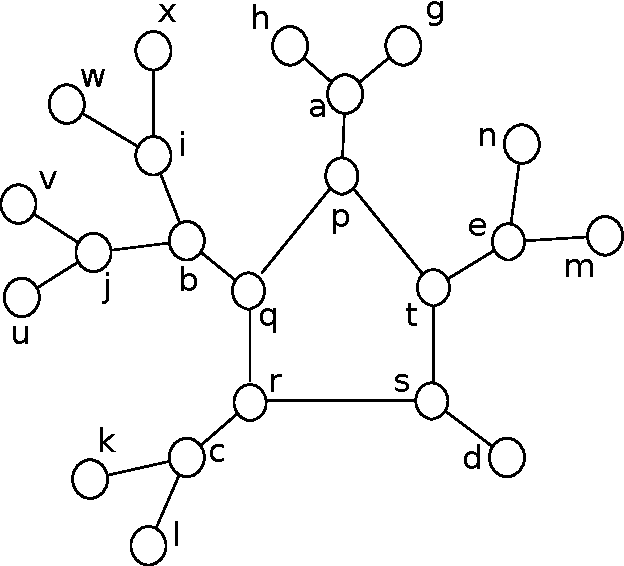
\includegraphics[scale=0.4]{pent} 
% \caption{Pentagon $pqrst$}
% \label{fig:pent}
% \end{center}
% \end{figure}



\section{}


\begin{table}
\centering
\begin{tabular}{| c | c |}
\hline
{\bf item 1} & {\bf item 2} \\ \hline
%
abcde & 5 \\ \hline
%
pqrst & 4 \\ \hline
\end{tabular}
\caption{A sample table}
\label{table:1}
\end{table}

\chapter{Introduction and Related Work}

%Replace \lipsum with text.
% You may have as many sections as you please. This is just for reference.

In this section, we will present the basic concepts necessary for understanding the Network virtualisation and the work that we will be presenting afterwards. We will start with concept of Virtualisation in general, subsequently moving onto the network virtualisation, software defined networking (SDN), virtual network management schemes in data centers and other related things.

\section{Virtualisation}
Virtualisation is the process of creating logical computing resources from available physical resources. It provides an abstraction layer between workloads and the underlying physical hardware by means of virtualisation software. The virtualised computing resources such as CPUs, storage, network, disk I/O, memory are pooled. These are then provisioned to workloads without worrrying about physical location within a data centre.

It also provides encapsulation so that workload can access only the resources assigned to them. In this way several independent workloads can be supported in a virtualised system.

\subsection{Types of Virtualisation}
Various virtualisation technologies are as follows:-

\begin{itemize}
    \item \textbf{Server Virtualisation} - it provides abstraction to the server physical computing resources from logical resources that are created. The user specifies the number of CPUs he requires and it is the virtualisation layer that maps it to the actual physical hardware. It increases the server utilisation.
    \item \textbf{Storage Virtualiastion} - it abstracts and pools the storage physical resources among workloads, thereby increasing storage utilisation. The user can specify the number and size of hard disk as part of parameters of it.
    \item \textbf{Network Virtualisation} - it allows to have multiple small logical network from large physical network and provision of large logical network from these multiple small networks. Network administrators can improve network traffic control, and security using network virtualisation.
\end{itemize}

\subsection{Benefits of Virtualisation}

There are several advantages of Virtualisation. Major ones are stated as:- 

\begin{itemize}
    \item \textbf{Save Expenditure} Network virtualisation gives consolidation of the resources. Therefore, less hardware is required hence it saves both capex and opex. The percentage through which utilisation of the resources can be increased is nearly 80\%
     \item \textbf{Provision of Network much faster} It offers faster provision of the network topologies. Unlike hardware assembly, ready templates can be designed for faster provision. They can be used when requested
     
      \item \textbf{Improved Disaster Recovery} The abstraction provided by the virtualisation enables us to use any commodity hardware, which makes possible to use cheaper hardware to built backup facility which is rarely used. Hence reduction in overall cost.
      
       \item \textbf{Utilisation of Resources} It has been found that on an average most of the systems operate at less than 15\% of their full capacity. Virtualisation increases this efficiency by making utilisation upto 80\% of the full capacity
        \item \textbf{Centralisation of Management} Administration becomes easy with virtualisation as it comes with the centralised and remote management
\end{itemize}


\section{Network Virtualisation}
The purpose of virtualisation is to simulate hardware services in software. All functionalities such as storage (in case of software defined storage) or network resources (in this case) are separated from the hardware and simulated in the software. The hardware platform can be any off the shelf general platform which allows for a more portable, scalable and cheaper solution.

When a network is virtualised, it creates a logical software-based view of the actual physical network and the functionalities of the network hardware boxes like routers, switches, etc. are implemented in the software itself. In this case physical device is only responsible for forwarding the packets, acting like a dumb switch, and all the routing and forwarding decisions are taken by the software.

Azodolmolky et. al. \cite{azodolmolky2013sdn} have studied different implementation of virtualization technologies and the table below summarizes the pro and cons of these technologies.

Traditionally, network virtualization has been implemented through the vir-
tual segments called VLANs. But these are limited in number to 4096 and
therefore scability is an issue.
We can categorise differenct techniques of network virtualisaton based on architechture listed below

\begin{enumerate}
    \item Hypervisor having dumb virtual switch plus normal physical switch
    \item Hypervisor having dumb virtual switch with intelligent physical switch
    \item intelligent virtual switch is provided with typical (L2/L3) physical switch
\end{enumerate}

Table 2.1 lists different Network virtualisation Technologies. We will discuss some of these technologies. 
\subsection{VLAN based virtualisation}
This is the traditional method of network virtualisation. In this technology, virtual segments are created which act as actual LAN segments. These offer applications like isolation and security etc. These are limited to 4096 and hence they are not scalable.

\subsection{VM-aware networking}
VM-aware VLAN based implementation scales better. Here the basic idea is
that the VLAN list on the physical switch to the hypervisor link is dynamically
adjusted based on the server need.

\subsection{VCDNI} Its principle is based on a virtual distributed switch, isolated from the rest of the network. It is controlled by vCloud director and used MAC-in-MAC encapsulation instead of VLAN. Therefore VM MAC address not visible in physical network. Here 4k limitation of VLANs is no more intact because of longer header in vCDNI protocol.


\begin{table}
\centering
\begin{tabular}{| p{6em} | p{5em} | p{1cm} | p{1cm} | p{5em} | p{5em} | p{5em} |}
\hline
{\bf Technology} & {\bf Bridging} & {\bf All host flooding } & {\bf vNet flooding} & {\bf VLAN 4k limit} & {\bf VM MAC visible} & {\bf State kept in network}\\ \hline
%
VLANs & Yes & Yes & Yes & Yes & Yes & Yes \\ \hline
%
VM-aware networking & Yes & No & Yes & Yes & Yes & Yes \\ \hline
vCDNI & Yes & Yes & Yes & No & No & MAC of hypervisors \\ \hline
VXLAN & No & Only to some hosts & Yes & No & No & Multicast groups \\ \hline
Nicira NVP & No & No & Some & No & No & No \\ \hline
\end{tabular}
\caption{Different network virtualization techniques}
\label{table:1}
\end{table}

\section{Software Defined Networking}
\subsection{Overview}
Software defined networking is referred to as the splitting of the network plane into a data plane and a control plane. The control plane consists solely the control logic and controls several devices in the data plane. The data plane, on the other hand, solely consists of forwarding logic such as switches. The control plane is considered to be dumb as it just forwards packets based on the instructions given by the control plane.

\subsection{Need for SDN}
Software defined networking is a framework which allows network programmers to automatically manage and control a large number of network devices, services, topology, traffic paths using high level languages and APIs. SDN pulls out the abstractions and allows one to look at the bigger picture. 
\begin{itemize}
    \item Virtualization: It is use of network resources without worrying about where it is physically located.
    \item Orchestration: Ability to control and manage thousands of devices with a few commands.
    \item Programmable: Ability to change behaviour dynamically without the need to suspend services.
    \item Visibiltiy: It allows the monitoring of resources and figure is the network is disrupted or the presence of any faults.
    \item Performance: It also allows traffic engineering (bandwidth management), load balancing, high utilization and error handling.
    \item Multi-tenancy: The tenants have a complete control over their addresses, topology, routing and security.
\end{itemize}

\begin{figure}[h]
\begin{center}	
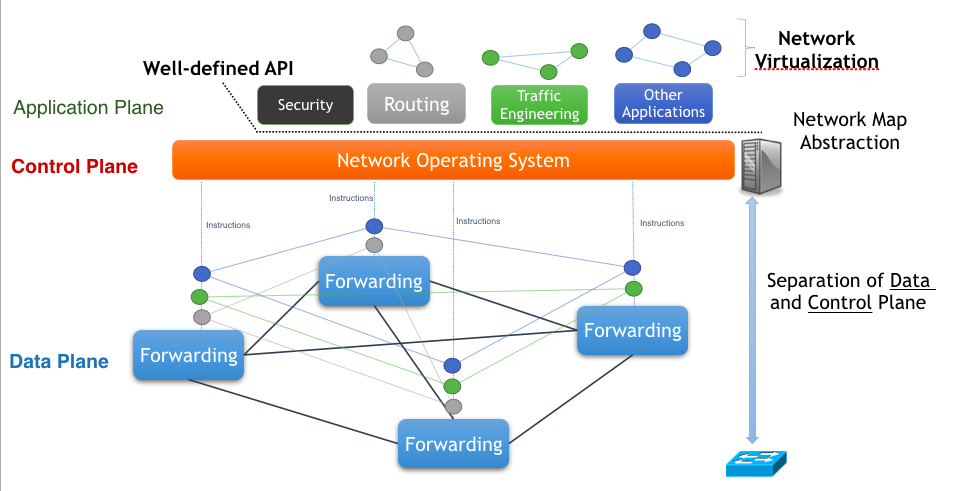
\includegraphics[scale=0.4]{data_control_plane} 
\caption{Separation of data and control planes }
\label{fig:data_control_plane}
\end{center}
\end{figure}

\subsection{Data and Control planes}
SDN consists of two separate planes which are data plane and control plane. In the traditional network where the forwarding logic is distributed to in the network. One example of this type of distribution is in the linked state routers where routers exchange information with each other to jointly create and image of the network while none of them have the complete view of the network. Unlike the traditional network, in SDN, the network intelligence is and states are logically abstracted out. The underlying network infrastructure is abstracted out from applications.
\begin{itemize}
    \item Data plane: The forwarding logic like switches run of general purpose commodity hardware. It is decoupled from specific networking hardware
    \item Control plane: The data plane is controlled, maintained and programmed from a central entity called a control plane 
\end{itemize}

\begin{figure}[h]
\begin{center}	
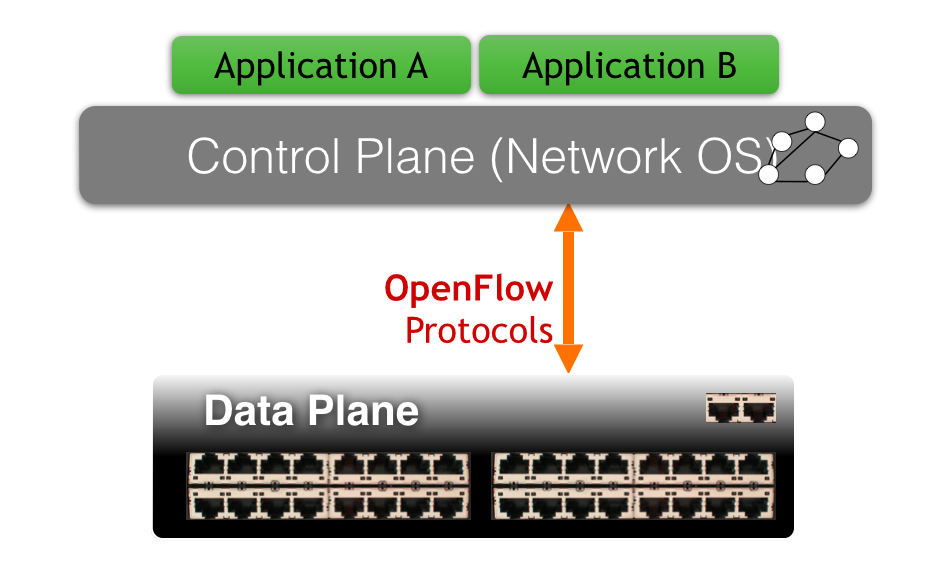
\includegraphics[scale=0.4]{openflow} 
\caption{OpenFlow}
\label{fig:openflow}
\end{center}
\end{figure}

\subsection{OpenFlow}
OpenFlow is a software defined networking standard.It allows network programmers to determine the path of network packets through a network of switches. It is a communication interface between the control plane and data plane of an SDN architecture. It allows direct access to as well as manipulation of the forwarding plane of network devices such as switches, routers, both physical and virtual. It can also be thought as a protocol for switches and controller interfaces.

\subsubsection{Working of OpenFlow}
OpenFlow manages the traffic (network flows) by manipulating a flow table at switches. Instructions are stored in flow tables. When a packet arrives at a switch, it matches the header fields with flow entries in a flow table. If any entry is matched, it performs indicated actions and updates the counters. If, however, it is not matches then the switch asks the controller by sending a message with the packet header.

% \subsubsection{OpenFlow table}
% The basic actions in an OpenFlow table are as follows:
% \begin{itemize}
%     \item All: To all interfaces except the incoming interface.
%     \item Controller: Encapsulate the packet and send it to the controller.
%     \item Local: Send to its local networking stack
%     \item Table: Perform actions in the next flow table 
%     \item In\_port: Send the packet back to the input port.
%     \item Normal: Forward in accordance with the traditional ethernet.
%     \item Flood: Send along the minimum spanning tree except the incoming interface.
% \end{itemize}

\subsection{SDN Controller}
SDN controller is a software which communicated to the hardware switches using the above mentioned OpenFlow protocols. A controller creates rules as to how a packet must be forwarded and installs these rules in hardware switches. A switch then simply forwards the packets according to the rules set up by the controller.

Now we briefly give a description of different SDN controller that are available today.

\subsubsection{Nox}
Nox was the first SDN controller that was developed. It is a C++ based controller and many other controller like pox have been developed over it. It is not in development now.

\subsubsection{Pox}
Pox is developed over Nox controller. It is a simple to use python based controller which can be used for rapid protyping of any SDN application.

\subsubsection{Ryu}
Ryu is a component based SDN framework with a well defined API. It supports various protocols other that OpenFLow like Netconf, OF-config.

\subsubsection{OpenDaylight}
OpenDaylight is an open source Java based project under Linux distribution. It has a huge community and contributors to its code base. Although a bit difficult to learn, it has a wide variety of features and is also used for commercial products.

\subsubsection{Floodlight}
Floodlight is also a Java based controller that we have used for developing our application. It has a growing community of developers and provides a rich set of northbound and southbound APIs to create an application module. 

\section{Baadal: IIT Delhi's Private Cloud}
"Baadal is a cloud orchestration and virtualization management software developed at IITD that can work with multiple virtualization technologies like KVM, Xen, and VMWare" \cite{baadaliitd}. Its main features include
\begin{itemize}
    \item Dynamic resource scheduling and power management
    \item An integrated work flow system for request of virtual machines
    \item Virtual machines can be powered on, powered off, resumed or suspended as per user requirement.
    \item Different costs for resources for VMs depending upon the requirement.
\end{itemize}

Currently Baadal is deployed in IITD on 48 blade servers with 500 cores and 50 TB of storage (which is virtualized storage based on Network attached storage or NAS). Out of these over 60 machines are being used for high performance computing in the campus.

According to \cite{baadaliitdwebpage} the technical specification of baadal are as follows:
\begin{itemize} 
    \item 32 blade servers with 2x6 core Intel(R) Xeon(R) CPU X5670 @ 2.93GHz and 16 GB RAM.
    \item 16 blade servers with 2x4 core Intel(R) Xeon(R) CPU E5540 @ 2.53GHz and 12 GB RAM.
    \item A 10Gbps ethernet backbone.
    \item 50 TB of virtualized storage on a NetApp 3210V NAS and HP EVA6400 SAN with FC disks.
    \item Open source virtualization technology based on KVM.
\end{itemize}

\subsection{Baadal sandbox}
To facilitate easy development and testing of application for use in Baadal deployment this sandbox environment is provided. It simulates the actual baadal architecture and configuration in a single machine without using any more physical hosts. Once an application is tested on this sandbox then it can be ported on the actual Baadal with little modifications.

\subsection{Netmap}
Netmap is a framework for high speed packet I/O. It is implement as a single kernel module and supports access to network cards, host stack, virtual ports and netmap pipes. 
It uses optimizations like batch processing of packets and using a circular queue as both input and output buffers. This reduces packet processing delays and eliminates copying delays.


\section{Related Work}
\subsection{SDN based Scheme for Virtual network management}
As we have seen in virtualisation services like storage, network, computing are provided using cloud. It required usage of virtual network. As part of this project, we suggested some of the changes in virtual network management schemes. But before moving onto the changes suggested and implemented we should have an idea of management schemes for the virtual network.
\begin{itemize}
    \item Three important aspects of management scheme are how to transfer virtual network packets, tenant isolation and adaptability of virtual network to topology changes.
    \item Considering these three factors management scheme can be divided into two types. One is \textbf{traditional bridging} which binds VMs NIC with physical NIC on a virtual bridge and transfer VMs packets via the physical NICs. This has advantage of good performance but it lacks flexibility.
    The other type based on \textbf{overlay network} which encapsulates the virtual network packets into the hosts packets. It has advantage of flexibility but it leads to performance loss.
    \item Using above two traditional methods we have to make a trade off between flexible management and network performance. But SDN allows us to accomplish management logic conveniently which helps to  achieve both flexibility and performance improvement.
    \item We have designed management scheme for vlan solution inspired from a scheme known as FENet.\cite{liu2014fenet}. FENet is SDN based approach for management scheme, creates virtual network upon devices which support OpenFlow protocol and SDN controller programs are developed to manage them.
    \item It provides improved network utilisation and lower latency than the scheme based on traditional bridging.
    \item Nicira Network virtualisation platform (NVP) provides a solution which combines idea of SDN and IP tunnelling. One of the other solution proposed for tenant isolation based on SDN, is conditional on the fact that hosts are in the layer 2 network.\cite{nunes2013virtualized}. It replaces the packet destination destination MAC address with the host MAC address while the destination IP address is still the VM's so that the packet routing does not happen across the physical network.
\end{itemize}

\subsection{Online traffic aware virtual machine placement in data center networks}
Dias et. al.\cite{dias2012online} have presented a virtual machine placement (VMP) algorithm to reallocate virtual machines in the data center servers based on the current traffic matrix, CPU, and memory usage. VMP takes into account the current data center work load, CPU and memory usage of virtual machines to avoid bottlenecks. The basic idea is to consolidate virtual machines that have correlated services. VMP operation is divided into four parts:

\begin{itemize}
    \item Data acquisition: The traffic between each pair of virtual machines is used to create a traffic matrix. It also takes the CPU and memory usage of each virtual machine as input as well as the topology of the data center. The most used topologies used are similar as all of them have a core which is responsible for connecting big segments of the network. Traffic engineering tries to push the traffic to the edges of the network thereby reducing it in the higher layers. 
    \item Server partitioning: They also have proposed an algorithm for partitioning of servers. The servers which have high degree of connectivity are clubbed together. Most suitable candidates for this type of aggregation are the servers which are placed at the same layers.
    \item Clustering virtual machines: They \cite{dias2012online} have used a community finding algorithm to find communities withing the virtual machines which clusters the virtual machines into groups which have high degree of connectivity.
    \item VM assignment: In the final step the virtual machines (which are clustered into communities by now) are allocated server partitions which were obtained in the server partitioning step.
\end{itemize}
In the simulations they have shown that their method is scalable to big data centers and provides an improvement of 12.5\% over no management.

\subsection{Traffic Engineering}
Jiang et. al. \cite{jiang2012joint} have proposed a solution to the problem of network load balancing by means of a joint tenant placement and route selection by exploiting multipath routing capability and dynamic virtual machine migration. They have proposed an offline algorithm that solves a static problem given a network snapshot, and an online solution for a dynamic environment with changing traffic. They have leveraged the technique of Markov approximation what required a very small number of virtual machine migrations. In simulations done by them they have evaluated the performance of online algorithms with real workload obtained from large computing clusters and have shown that their algorithm incurs the minimum performance cost in comparison to all other tested algorithms.

Biran et. al. \cite{biran2012stable} have also studied this problem and said that VM placement should consider the aggregate resource consumption of co-located VMs in order to obey service level agreements at lower possible cost. Also, the traffic patterns are not stable in nature and vary over a period of time. They have addressed this problem by trying to allocate a placement that not only satisfies the predicted communication demand but also is resilient to demand time-variations. They have defined the problem as a min cut ratio-aware VM placement which is NP-hard in general but they have employed several heuristics to solve it. Through their simulations they have shown that the placements based on their algorithm increase data scalability, while being able to support time-varying traffic demands with a reduced number of dropped packets. 

\subsection{Network Function Virtualization}
Middleboxes like proxy servers, firewall, NAT, etc. have become indispensable for today's networks. However, they come with problems like being expensive, difficult to manage and scale. Many of these problems arise because of the fact that they are hardware based devices. As a solution to this problem a recent trend toward Network Function Virtualization has started to turn these middleboxes into software-based entities.

Matins et. al. \cite{martins2014clickos} have introduced a virtualized software middlebox platform called ClickOS. It is based on Xen sice it provides para-virtualized VMs to build a low delay and high throughput platform. Through their evaluation they have shown that ClickOS can hundreds of middleboxes on commodity hardware, offers millions of packet per seconds processing and provide low packet delays. They have shown that even low-end servers can forward packets at 30Gbps. 

Ge et. al. \cite{ge2014openanfv} have built a consolidated framework OpenANFV for speeding up the performances of virutalized middleboxes. When a middlebox is needed its resources are orchestrated by OpenStack and is instantiated as a virtual machines on a common platform. They have a Network Functions Acceleration Platform (NFAP) which provides a FPGA card which accelerates various functions. In their evaluations they have shown orders of magnitude of improvement in throughput in virtualized middleboxes like deep  packet inspection, network address translation, etc. using NFAP as compared to without NFAP.

Han et. al. \cite{han2015network} have  explained the requirements, architectural framework and use cases for NFV and have also discussed the challenges in this area. They argue that although virtualization impacts performance negatively in terms of throughput and latency, these effect must be kept to a minimum. Migrating from the existing architecture to NFV based solution is also a major hurdle that network carriers face. They have presented a architectural framework for NFV which includes four components - orchestrator, VNF manager, virtualization layer and virtualized infrastructure manager. They have also given various use cases for NFV like virtualization of cellular base station, virtualization of cellular core network and virtualization of home network.

\chapter{Simulation tools and Introduction to Baadal Architecture}

Getting started with theory of Software defined networking, we tested our grasp on literature by performing simulations with basic topologies and scripts. 

For basic experimentation, we started with the mininet for creating customised topologies using python scripts. Later on we created the baadal architecture using physical host (baadal sandbox).
We will also discuss the baadal networking architecture as a prerequisite to move forward with the installation of baadal sandbox and further development.

\section{Mininet}

Mininet is a network emulator. It creates a network of virtual hosts, switches, controllers, and links. It runs standard Linux network software and supports OpenFlow for flexible custom routing and software defined networking. Some of the features of mininet are: 
\begin{itemize}
    \item A simple and inexpensive \textbf{network testbed} provision for developing OpenFlow applications
    \item enables complex topology testing, without the need to wire up a physical network
    \item enables multiple concurrent developers to work independently on the same topology
    \item provides an extensible Python API for network creation and experimentation
\end{itemize}

\section{Overview of Baadal Networking Architecture}
In this section we will present the overview of the baadal networking architecture. The components comprising the architecture are mentioned below:-

\begin{itemize}
    \item \textbf{NAT} Network Address tanslator is the component which act as firewall for the baadal network. All the traffic of the baadal network pass through it. Internal baadal nodes communicate to the internet via this interface only. It is implemented on an OpenVswitch which is hosted in a physical machine with Ubuntu as its OS.
    \item \textbf{Hardware Switch} It is a physical switch which is connected to all the other networking components including the physical hosts, Baadal Controller, Filer and NAT.
    \begin{figure}[h]
\caption{Overview of Baadal Architecture}
\centering
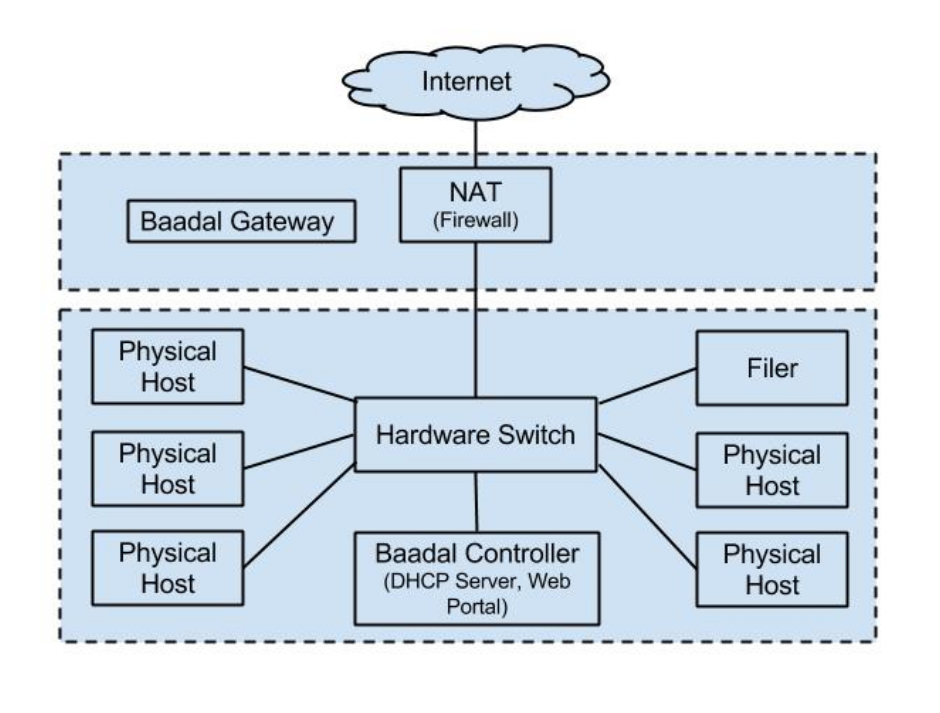
\includegraphics[width=0.9\textwidth]{Baadal_architecture}
\end{figure}
    \item \textbf{Baadal Controller} This component is responsible for providing web portal where a user can request a VM, a facutly supervisor approves it and an administrator can commission it. The main function of it is to be central controlling element alongwith hosting components like DHCP server, TFTP server, scheduler etc.
    
    \item \textbf{Filer} For all the physical hosts Filer is the network file manager. On request of virtual machines, controller hosts the virtual hard disk. But additional hard disk is allocated in the filer machine.
    
    \item \textbf{Physical host} These are responsible for hosting all the VMs created by the user. KVM is the hypervisor layer in the physical host.
    
\begin{figure}[h]
\caption{Physical host architecture}
\centering
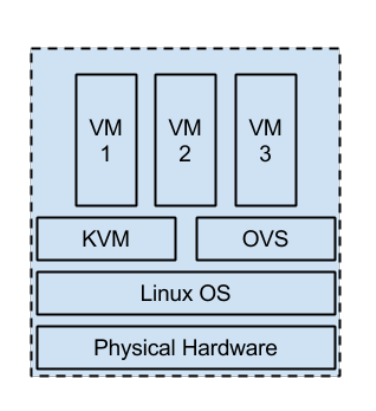
\includegraphics[width=0.5\textwidth]{PhysicalHost_architecture}
\end{figure}
\end{itemize}

%\section{Implementation of Virtual Network using OpenDaylight}

\chapter{Baadal Sandbox Setup Usage}

This chapter will provide the necessary commmands, interfaces and methodology to use baadal sandbox. We thought of including this as we spent much of the effort in understanding baadal system. There is no proper documentation on usage of baadal sandbox. Hence we put necessary screenshots in this chapter to enable others use baadal sandbox in convenient manner.

Following are the steps to start with sandbox server we established:-

\begin{enumerate}
    \item Login to server used for baadal sandbox setup
    
\begin{figure}[h]
\centering
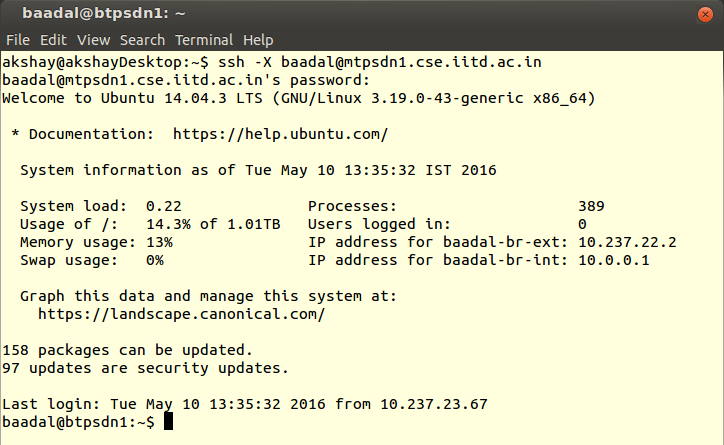
\includegraphics[width=0.9\textwidth]{first_login}
\caption{Login to the baadal sandbox server}
\end{figure}

\newpage
\item For status of VMs running in sandbox we can use \textit{sudo virsh list --all}
\begin{figure}[h]
\caption{Different VMs running in the sandbox}
\centering
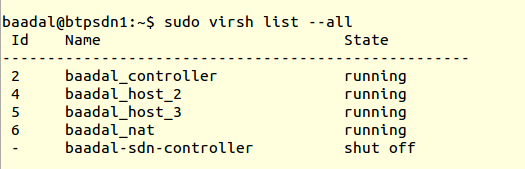
\includegraphics[width=0.9\textwidth]{Status_VMs}
\end{figure}


\item Using \textit{ifconfig} we can see the network configuration for the server.
\begin{figure}[h]
\caption{Output of ifconfig command on sandbox server}
\centering
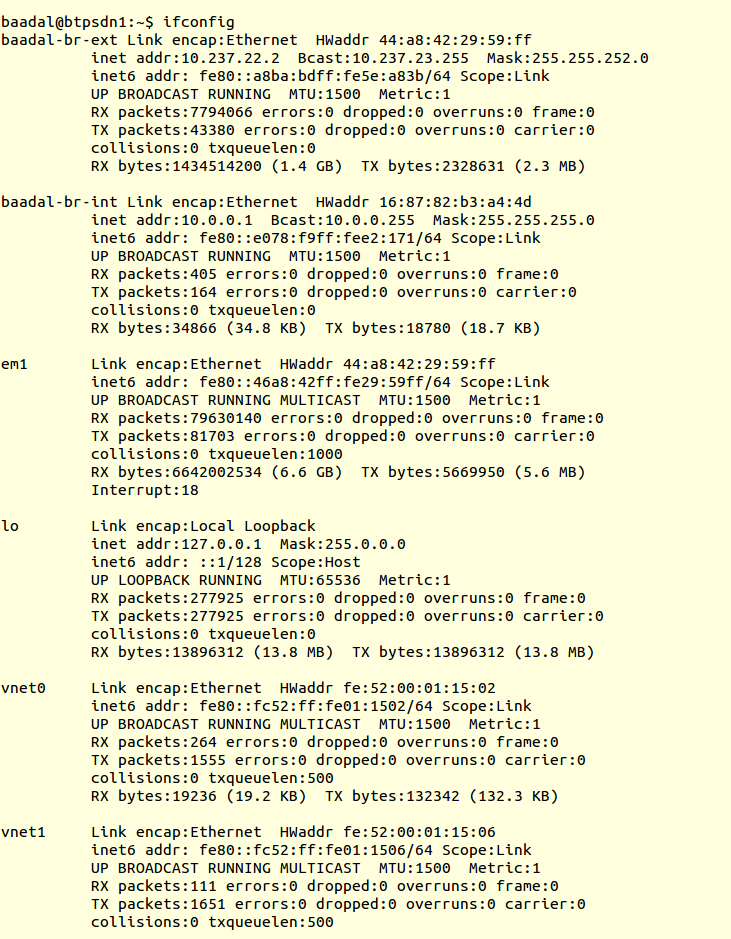
\includegraphics[height=10cm, width=0.9\textwidth]{ifconfig_server}
\end{figure}

\newpage
\item login inside the controller

\begin{figure}[h]
\caption{Login in the baadal controller}
\centering
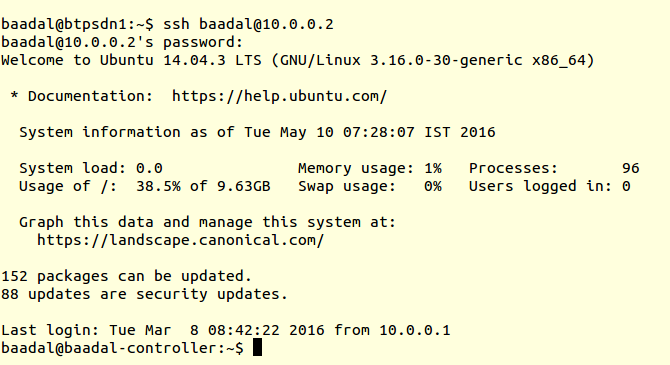
\includegraphics[height = 5cm, width=0.9\textwidth]{login_controller}
\end{figure}


\begin{figure}[h]
\caption{ifconfig showing 255 fake bridges inside the controller}
\centering
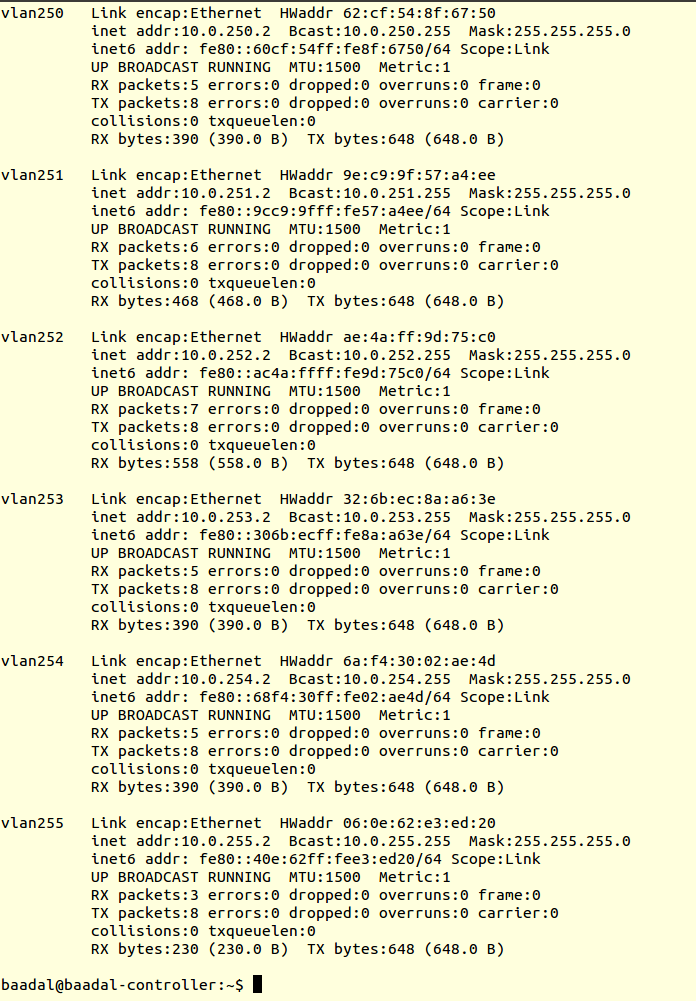
\includegraphics[height=9cm, width=0.9\textwidth]{ifconfig_controller}
\end{figure}

\begin{figure}
\caption{Web2py Processes Running inside controller}
\centering
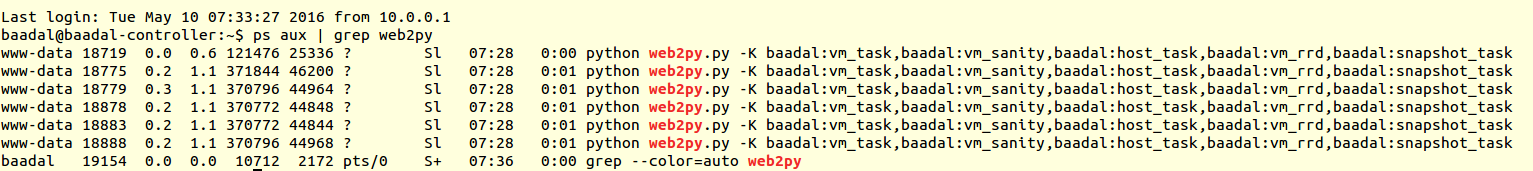
\includegraphics[height=2.5cm,width=0.9\textwidth]{web2py_processes_controller}
\end{figure}

\newpage
\item Login inside the nat is shown as

\begin{figure}[h]
\caption{Login inside the nat}
\centering
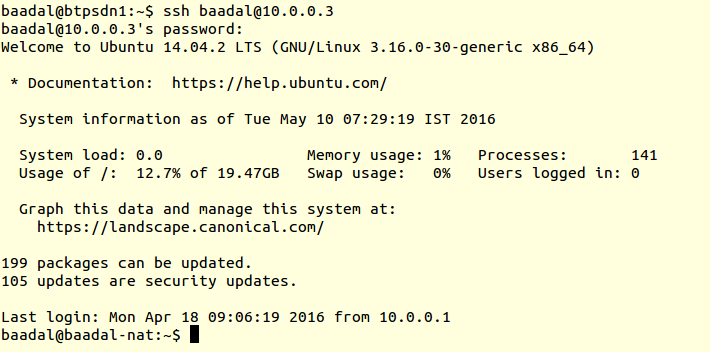
\includegraphics[width=0.9\textwidth]{login_nat}
\end{figure}


\begin{figure}[h]
\caption{ifconfig showing 255 fake bridges inside the NAT}
\centering
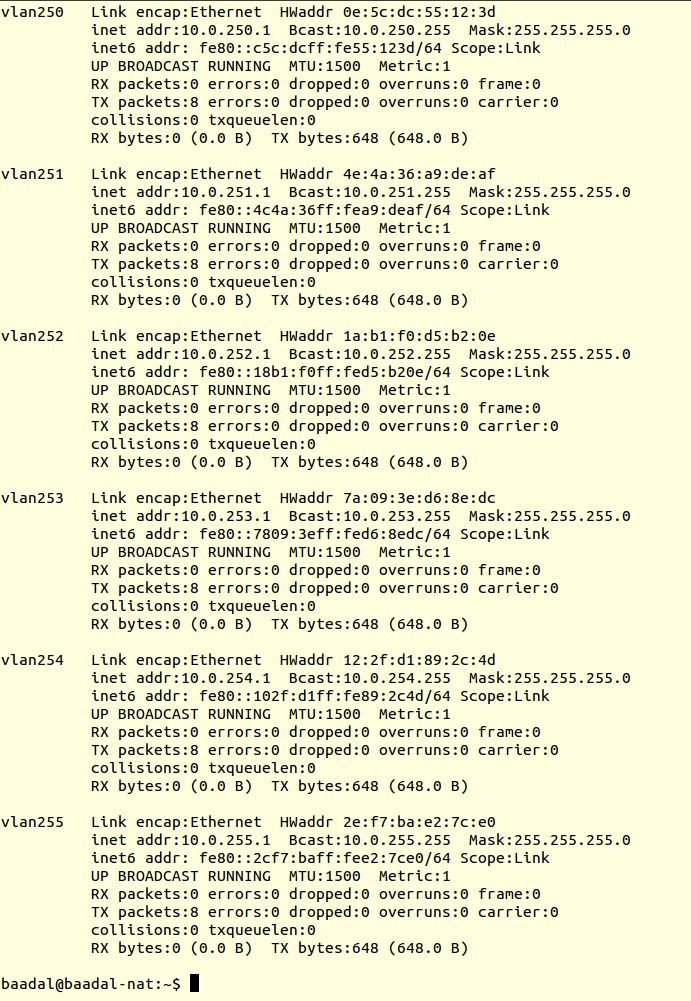
\includegraphics[width=0.9\textwidth]{ifconfig_nat}
\end{figure}

\item Login inside host

\begin{figure}[h]
\caption{Login inside host 10.0.0.6}
\centering
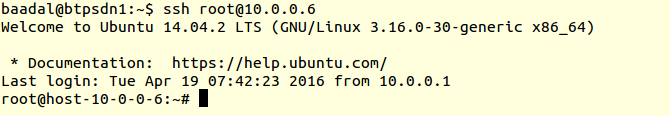
\includegraphics[width=0.9\textwidth]{login_host_6}
\end{figure}


\begin{figure}[h]
\caption{Network configuration of host 10.0.0.6}
\centering
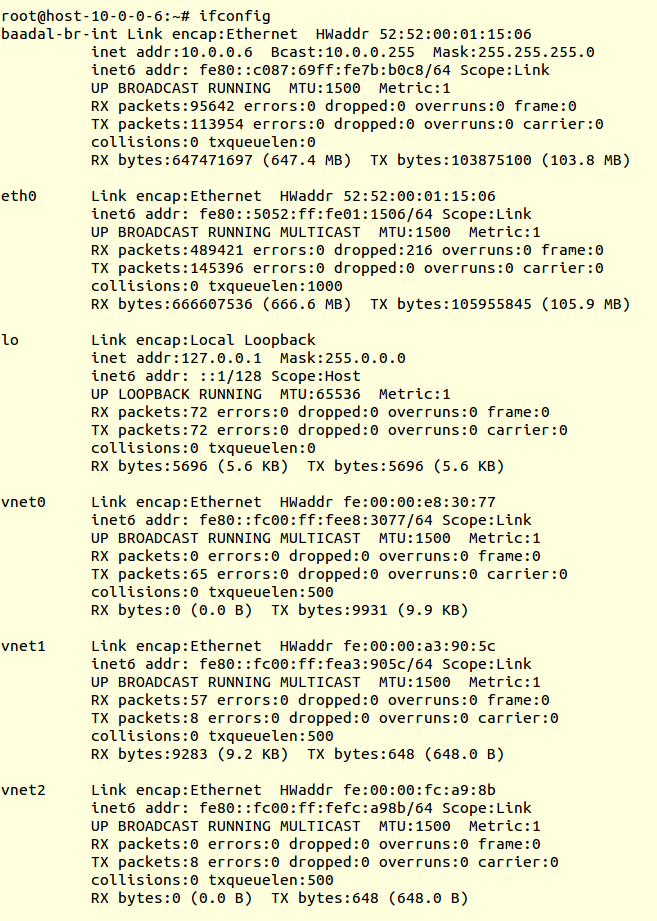
\includegraphics[width=0.9\textwidth]{ifconfig_host6}
\end{figure}

\begin{figure}[h]
\caption{Login inside host 10.0.0.7}
\centering
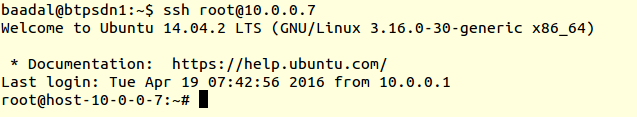
\includegraphics[width=0.9\textwidth]{login_host7}
\end{figure}


\begin{figure}[h]
\caption{Network configuration of host 10.0.0.6}
\centering
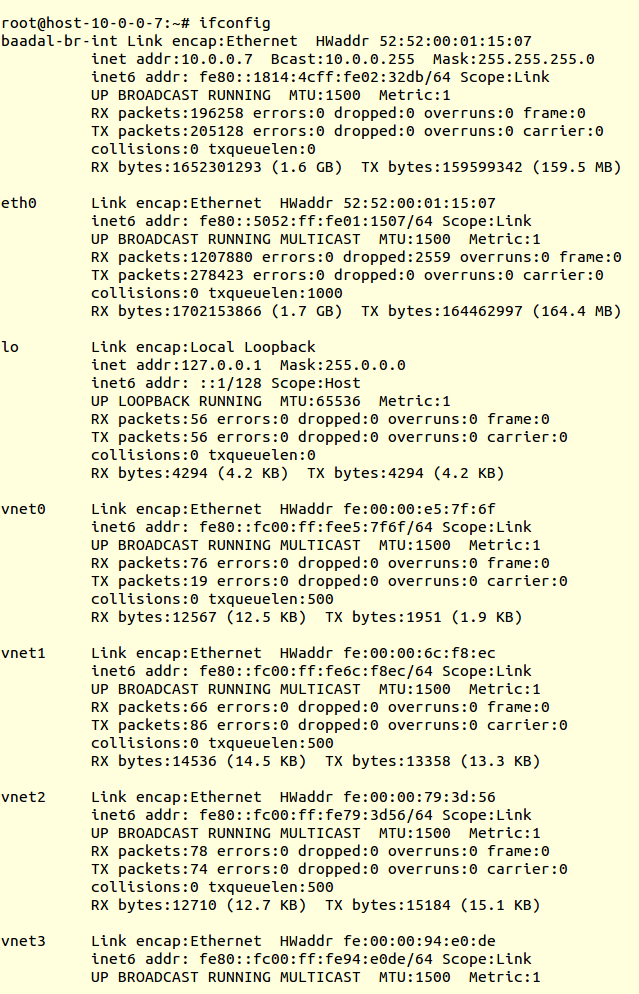
\includegraphics[width=0.9\textwidth]{ifconfig_host7}

\end{figure}

\item \textit{virsh list --all} shows the VMs running inside 10.0.0.6

\begin{figure}[h]
\caption{VMs shutdown status inside host 10.0.0.6}
\centering
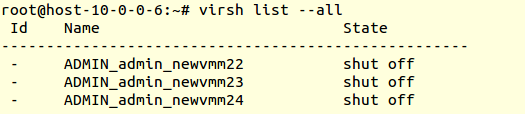
\includegraphics[width=0.9\textwidth]{host6_VMs_shutoff}

\end{figure}

\begin{figure}[h]
\caption{Starting VMs inside host 10.0.0.6}
\centering
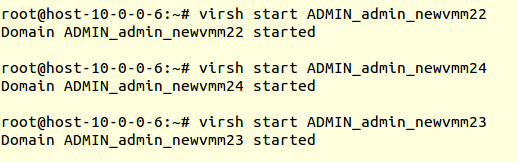
\includegraphics[width=0.9\textwidth]{host6_VMs_start}

\end{figure}

\begin{figure}[h]
\caption{Running VMs inside host 10.0.0.6}
\centering
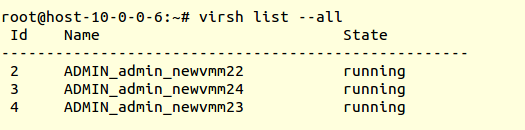
\includegraphics[width=0.9\textwidth]{host6_VMs_running}

\end{figure}

\item \textit{virsh list --all} shows the VMs running inside 10.0.0.7

\begin{figure}[h]
\caption{VMs shutdown status inside host 10.0.0.7}
\centering
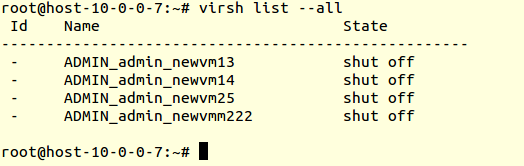
\includegraphics[width=0.9\textwidth]{host7_VMs_shutoff}

\end{figure}

\begin{figure}[h]
\caption{Starting VMs inside host 10.0.0.7}
\centering
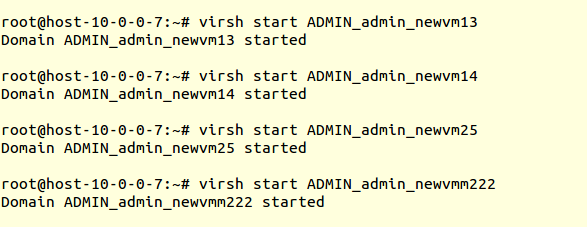
\includegraphics[width=0.9\textwidth]{host7_startinVMs}

\end{figure}

\begin{figure}[h]
\caption{Running VMs inside host 10.0.0.7}
\centering
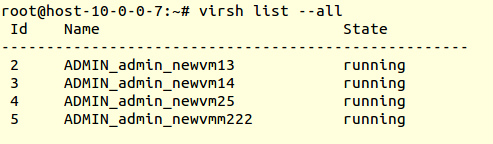
\includegraphics[width=0.9\textwidth]{host7_VMs_running}

\end{figure}

\item \textit{virt-viewer domain\_name} will open the GUI for the VM whose domain name is specified. Below figure shows for VM \textit{ADMIN\_admin\_newvm25}


\begin{figure}[h]
\caption{Console output for VM 10.0.4.25 after running virt-viewer}
\centering
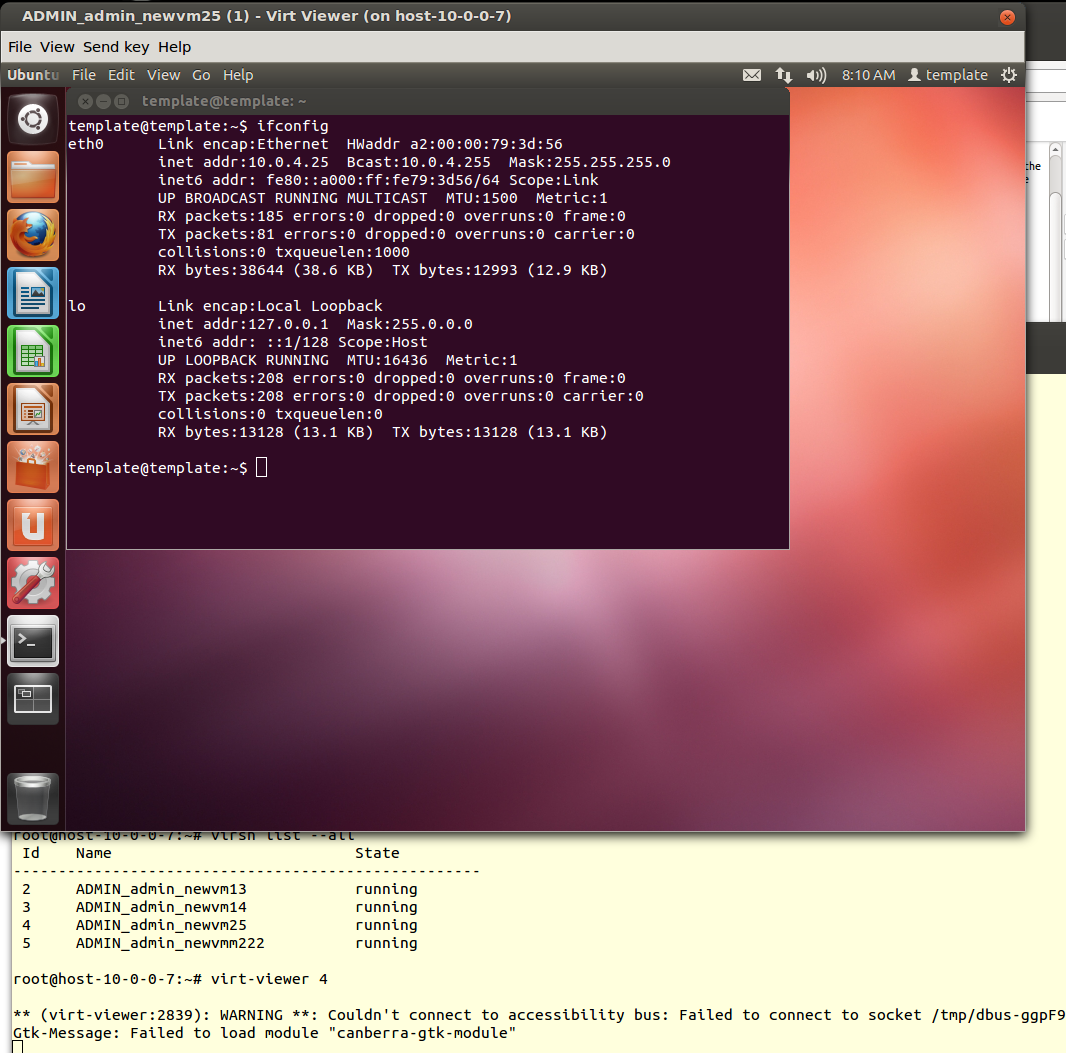
\includegraphics[width=0.9\textwidth]{virt_viewer_host7_ifconfig_425}
\end{figure}
\end{enumerate}

\chapter{Introduction to SDN based Application}

\section{Introduction to Floodlight}
Floodlight is an open source java-based SDN controller and was the controller of choice for this project because of reasons such as - it supports switches which are OpenFlow enabled, it is Apache licensed and can be used for almost any purpose, it has good documentation and a very active community of professional developers who were able to resolve any issues that we needed help with.


\section{Floodlight Architecture}
\begin{itemize}
\item OpenFlow – works with physical- and virtual- switches that speak the OpenFlow protocol
\item Offers a module loading system that make it simple to extend and enhance. 

\item Open community – Floodlight is developed by an open community of developers. It welcomes code contributions from active participants and openly share information on project status, roadmap, bugs, etc.

\item Easy to Use- Floodlight is drop dead simple to build and run. Read through the Documentation (link)

\item Tested and Supported – Floodlight is the core of a commercial controller product from Big Switch Networks (link) and is actively tested and improved by a community of professional developers


\end{itemize}
    
\begin{figure}[h]
\caption{Floodlight Architecture}
\centering
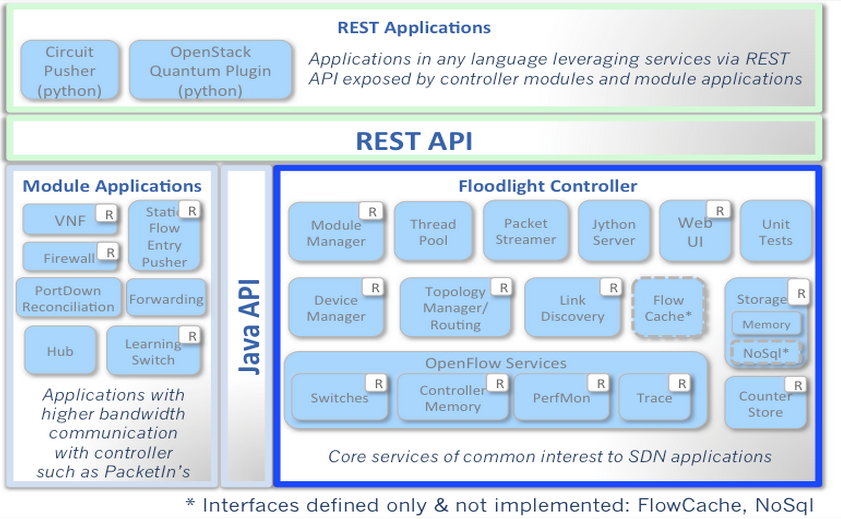
\includegraphics[width=0.9\textwidth]{Floodlight_architecture}
\end{figure}

\section{Baadal Sandbox setup}
For testing the simulation of the application, we need an environment like baadal. Baadal sandbox provides an environment by replicating actual Baadal architecture and configurations. It is fast and easy way to test the solution of network virtualisation. 



\begin{figure}[h]
\caption{Setup of Baadal Sandbox Installed }
\centering
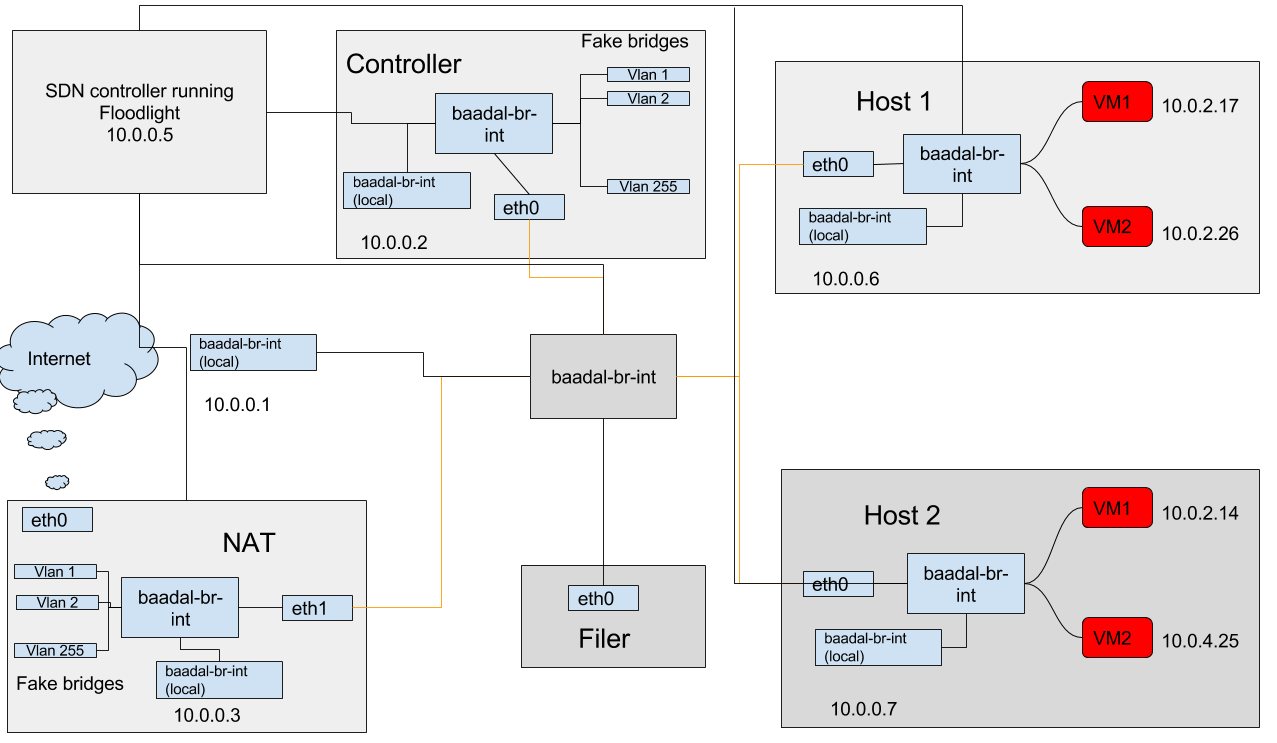
\includegraphics[width=0.9\textwidth]{baadal_networking_diagram}
\end{figure}

If tested successfully, we can subsequently deploy the solution in actual Baadal with some modifications.

The differences with which sandbox mimics baadal architecture are:-

\begin{itemize}
    \item Physical hosts, baadal controller, filer, NAT are implemented as VMs on a single physical machine
    \item OVS is the switch used for implementing hardware switches
    \item All the VMs are implemented into the physical hosts which makes two level of virtualisation
\end{itemize}



\section{Inter-VLan Issues and Modifications suggested}

\subsection{How do VMs communicate?
}
In the existing
Baadal network as explained above, the inter VM communication takes place
as follows:


\begin{itemize}
   
    \item \textbf{VMs in same host and same VLAN/subnet} In this case, the OVS bridge
in the host would simply be able to let them communicate by learning their
mac-port pair as they fall in the same broadcast domain. 

\begin{figure}[h]
\caption{Routing in Same Host and Same VLAN}
\centering
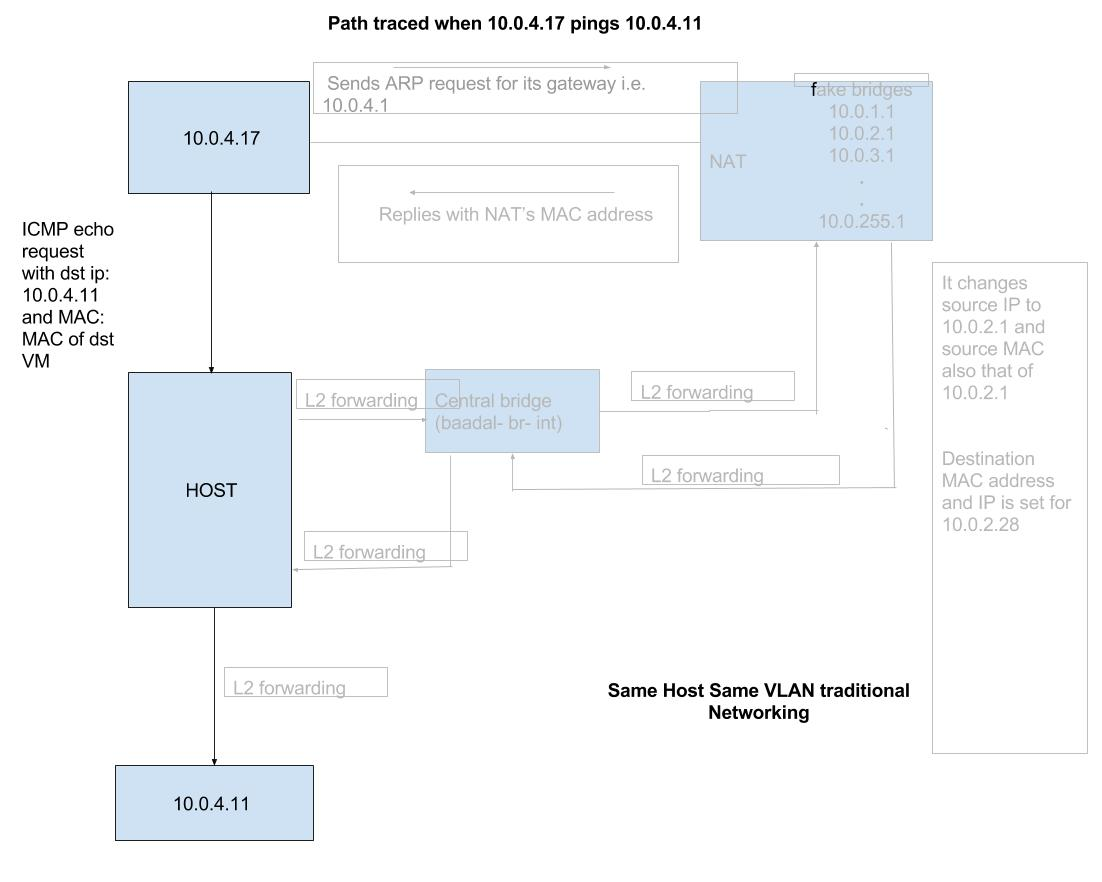
\includegraphics[width=0.9\textwidth]{Samehost_SameVLAN}
\end{figure}

The VLAN
tag corresponding to the VLAN will be attached at the ingress port while
the egress port will strip it off before sending the packets out.


\pagebreak



     \item \textbf{VMs in different host but same VLAN/subnet} In this case, still, the broad-
cast domain is the same. So, in addition to the host OVS bridge, the
central switch will come into picture. The process will be same as above
case except for the extra central switch through which the packets would
travel.

\begin{figure}[h]
\caption{Routing in Same Host and Same VLAN}
\centering
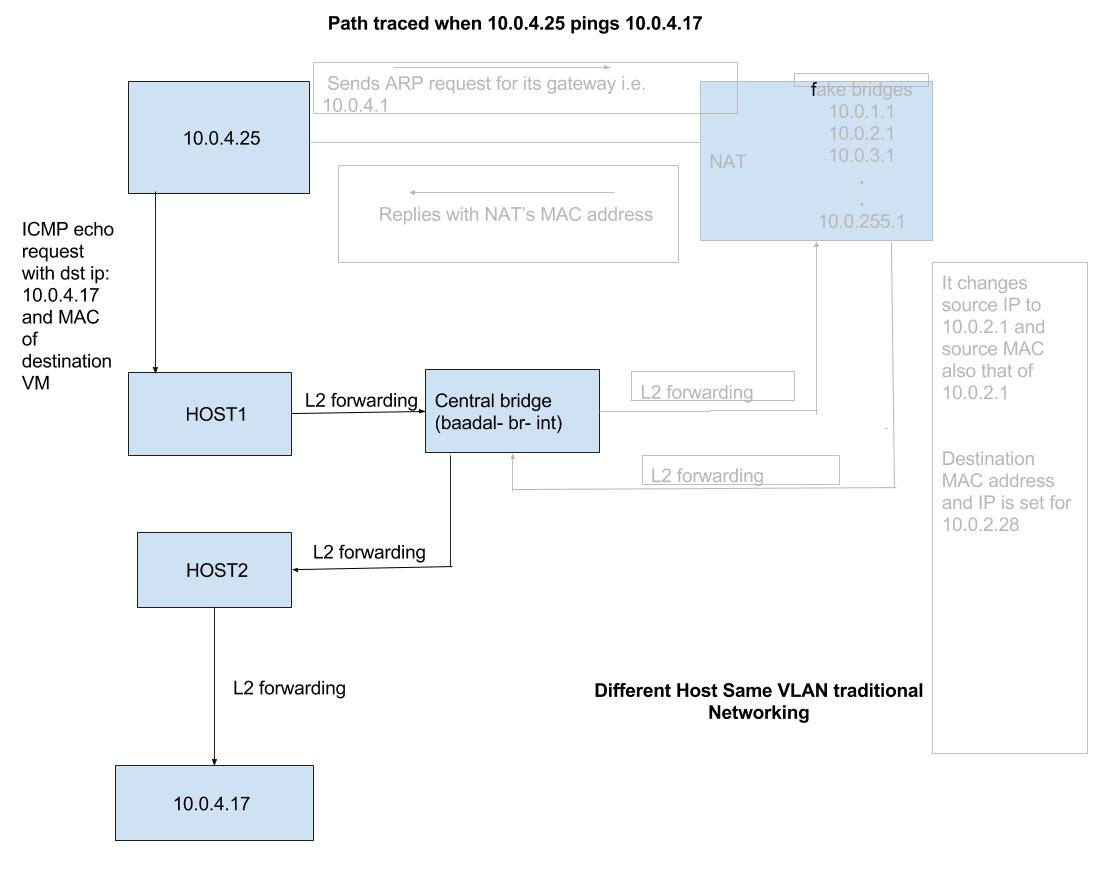
\includegraphics[width=1.0\textwidth]{Differenthost_sameVLAN}
\end{figure}

\pagebreak

      \item \textbf{VMs in the same host but different VLANs/subnets}The host OVS bridge,
in this case, would not be able to forward the packets as the broadcast
domains are different. As the gateway is fake bridge for that VLAN, the
packets go all the way up to the NAT machine passing through the central
switch. The fake bridges functions to modify the VLAN tag from the in-
put VLAN to the output VLAN. The modified packets are then forwarded
at the appropriate port of NAT OVS bridge and then they come back to
the same host. Finally, the OVS bridge in the host strip off the VLAN
tag and send it out the appropriate port.

\begin{figure}[h]
\caption{Routing in Same Host and Different VLAN}
\centering
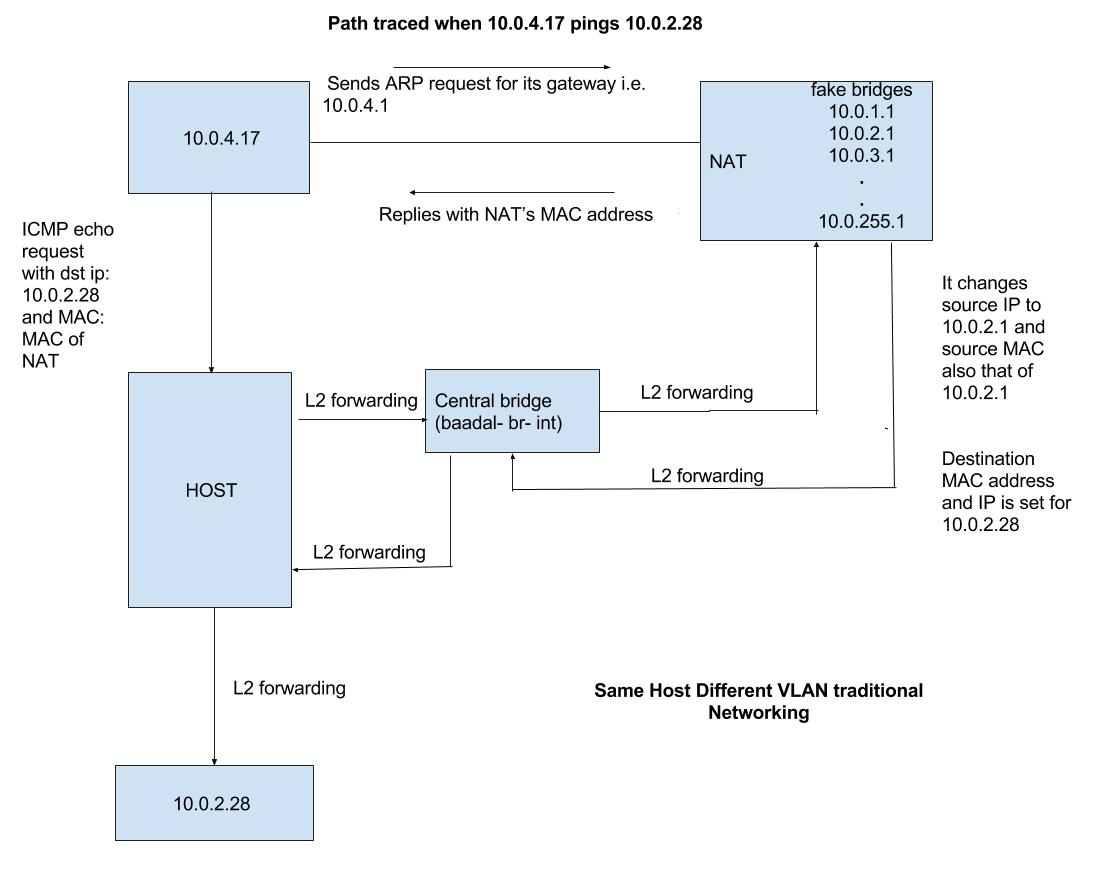
\includegraphics[width=1.0\textwidth]{Samehost_differentvLan}
\end{figure}

\newpage

\item \textbf{VMs in different hosts and different VLANs/subnets} the process is ex-
actly similar as in the previous case. The only change - different destina-
tion host - would be taken care off by the central switch as a part of its
normal l2-learning functionality.

\begin{figure}[h]
\caption{Routing in Different Host and Different VLAN}
\centering
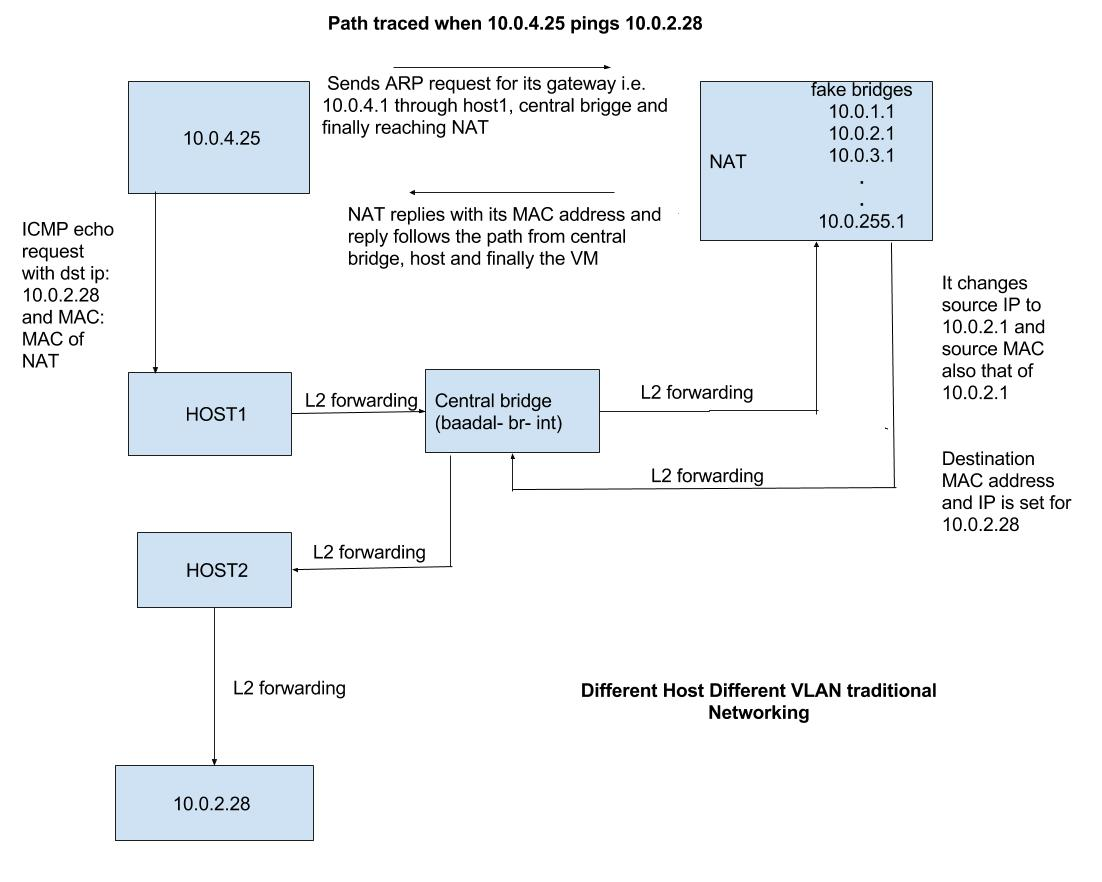
\includegraphics[width=1.0\textwidth]{Differenthost_differentvLan}
\end{figure}

\end{itemize}

\pagebreak 

\subsection{Limitation in present architecture}
We find the following limitations in the present architecture.

\begin{itemize}
\item Inter-VALN or subnet routing In the above architecture, fake bridges are
used as the mean to enable this feature. The issue is when VMs in the
same host but different subnet want to communicate. The packets have to
go all the way upto NAT machine and come back. This seems unnecessary
strain on the network and large latencies.

\item  Controlling inter-VALN routing Currently, there is no way of turning VLAN
routing on or off in Baadal. It is enabled by default. A granular level control of this feature with the current network architecture seems non-trivial
and difficult to implement



\item Maximum number of VLANs This architecture has an upper boung of 255
VLANs because of the one to one correspondence between the subnets
and the VLANs.


\item Number of VMs in a VLAN The number of VMs in each VLAN in the cur-
rent implementation is upper bound at 255. This is when considering the
addressing scheme of 192.168.x.y or 172.16.x.y with 255x255 addresses
available.

\end{itemize}

\subsection{Modification in Network Architecture}
We proposed and implementing the following modifications in the network architecture.

\begin{itemize}
    \item \textbf{No subnets} The reason subnets are used is because they define the broadcast
domains. The domains restrict the hops that broadcast packets travel and
helps in controlling traffic volume in network. But, with a SDN controller
application, the same thing could be acheived without having the subnet
restriction. The reason we want to remove it is bacause the fake bridges
are required only to enable inter subnet routing. Fake bridges being in
NAT requires packet to cover all the way upto NAT and back. Thus,
with just one subnet, the local OVS bridges would be able to forward the
packets.
\item \textbf{VLANs implemented using VLAN tags only} As opposed to having both
subnets and VLAN tags to implement VLANs, we use only VLAN tags.
The IEEE 802.1q protocol provides 12 bit VLAN tag amounting to 4094
tags. This would enable us to have 4096 VLANs as opposed to just 255!
We can further extend this to even larger numbers if we use both inner
and outer VLAN tags. Note that the VMs and the hosts are not VLAN
aware in the current as well as the proposed network architecture.

\end{itemize}

\section{Introduction to Policy routing application}
The virtual machines running in Baadal are allotted a security domain (a vlan) to segregate traffic of a certain vlan from other vlans. With using the traditional networking approach there is no way to disable it (inter-vlan routing is disabled by default in Baadal). With the SDN solution we have the capability to enable or disable it using a REST API. Moreover, there is also a provision for enabling/disabling communication between two virtual machines irrespective of their security domain. The use case for this feature would be a scenario in which people working with virtual machines in different vlans (because of them being in different departments or areas of the campus) need to collaborate with each other.

\section{Application that we are working on: Functionalities}

The application that we are working on implements modified network architecture as suggested above. The important tasks that will be handled in the application are as follows:

\begin{itemize}
    \item Tagging the packets if they ingress at an access port in a host and egress
from the trunk port.
\item Untagging the packet when they are to egress to an access port and they
have a tag attached

\item The application handles ARP and DHCP packets which are special kind
of packets. The details of how it is being done is presented in the following
sections.

\item The application takes care of security by restricting which kind of packets
reach where.

\item It takes care of forwarding normal traffic from one node to other.

\item It handles inter-VLAN routing as well.




\end{itemize}



\section{Floodlight modules}
Floodlight has modular architecture to implement any application over it and control its features. There are two kind of modules in floodlight
\begin{itemize}
    \item \textbf{Controller Modules} these implement core network services a software defined network should expose to applications
    \item \textbf{Application Modules} these implement solutions for different purposes like firewall, static flow pusher, L2 learning switch etc.
\end{itemize}

Module loading system has a JAVA interface IFloodlightModule that realises this framework.
\subsection{Module Loading System} The following are the objectives of the this system
\begin{itemize}
    \item What are the modules that are to be loaded using a configuration file
    \item Modify the implementation of modules without affecting other modules that are dependent on them
    \item Creating a platform and API to extend Floodlight
    \item Code Modularity is enforced
    \end{itemize}
The main parts of this system are 
\begin{itemize}
    \item \textbf{Modules} It is a class that implements the IFloodlightModule interface
    \item \textbf{Services} these are the services that the module provides. these are implemented as interface that extends the IFloodlightService interface
    \item \textbf{Configuration file} It contains the modules that are to be loaded
    \item \textbf{module file} It contains list of all classes used by JAVA service loader  
\end{itemize}

\subsection{How to write a Module} Following are main steps for writing a Floodlight Module
\begin{enumerate}
    \item Add a class to implement IOFMessageListener and IFloodlightModule interfaces
    \item Import Module Dependencies and set up Initialization
    \item Register a listener for PACKET\_IN Messages
    \item Ordering the modules for processing OpenFlow Messages before or after a particular module as required by the application
    \item Register the module in configuration file to load the module on startup
\end{enumerate}
    
\subsection{Module: Baadal}
It implements IOFMessageListener, IFloodlightModule, and IBaadalService. The data structures used are
\begin{itemize}
    \item \textbf{gateways} list of ipv4 addresses for routing between different subnets.  
    \item \textbf{ipToTag} stores mapping of ipv4 addresses to VLAN tags
    \item \textbf{interVmPolicy} Stores the status(enabled or disabled or default) of policy routing between a pair of VMs
    
\end{itemize}

The main functions implemented are 

\begin{itemize}
    \item \textbf{processPacketIn()} sends the packet for processing according to the source switch that it is coming from
    \item \textbf{init()} initialises variables and data structures (ipToTag, interVmPolicy etc.)
    \item \textbf{TimerTask()} schedules a task to clear cached entries in data structures at regular intervals
    \item \textbf{getIpToTag()} it returns mapping between IP address and corresponding VLAN tag
    \item \textbf{addIpToTag()} adds entries for mapping between IP address and VLAN tag
    \item \textbf{getInterVmPolicy} it returns the status of policy control for different pair of VMs
    \item \textbf{addInterVmPolicy} it adds entries into inter VM policy table as per requirement
    
\end{itemize}

\section{How do VMs communicate after implementation of application}

After running the policy control application, the modifications in the routing of different cases are  


\begin{itemize}
    \item \textbf{Same host and same VLAN} In this case routing design will be same as per traditional routing in baadal where the host will simply forward the packet based on the MAC address.
\end{itemize}


\begin{figure}[h]
\caption{Routing in Same Host and Same VLAN using SDN}
\centering
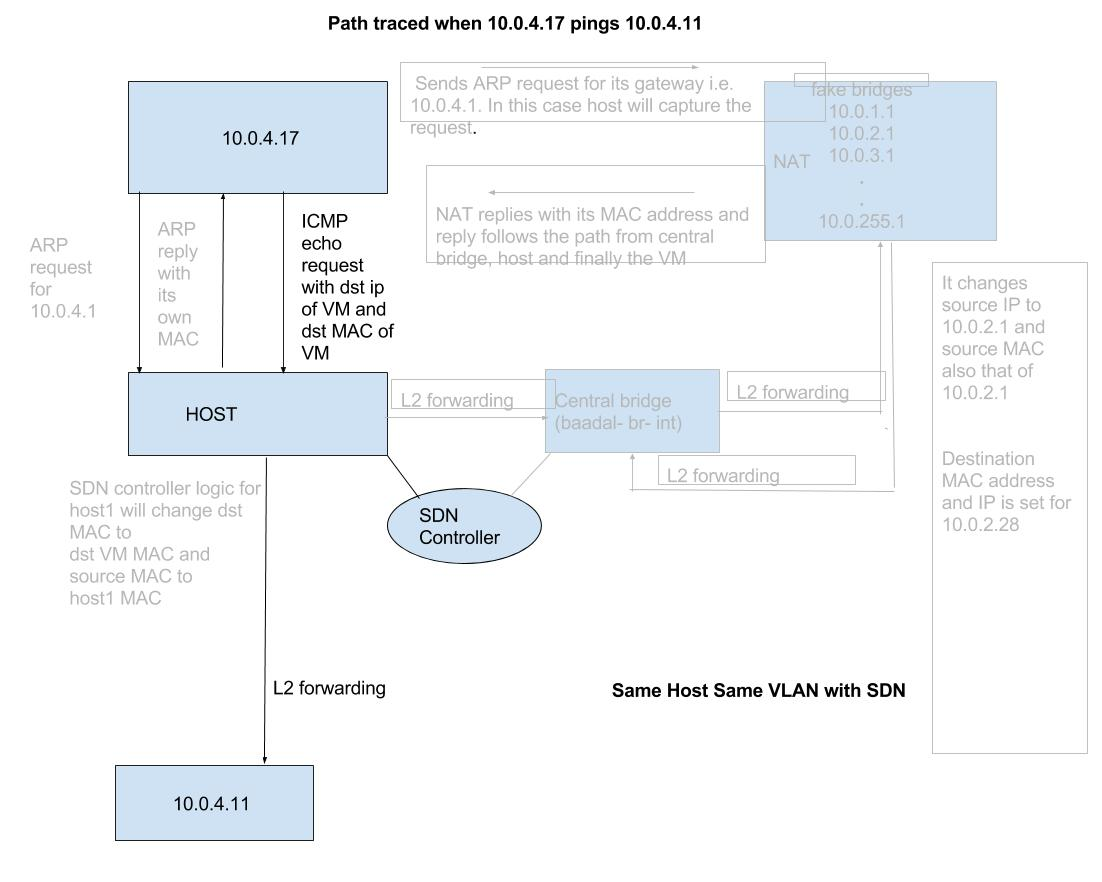
\includegraphics[width=0.9\textwidth]{Samehost_SamevLan_SDN}
\end{figure}

\pagebreak 

\begin{itemize}
    \item \textbf{Same host and Different VLAN} In this case host itself will reply to the ARP request, sent by the VM for its gateway. In traditional routing, this reply was generated by the NAT. Now the host will forward the packet to the destination VM by changing the ethernet frame (setting the destination MAC address to Destination VM MAC address and Source MAC address to MAC address of the host)
\end{itemize}

\begin{figure}[h]
\caption{Routing in Same Host and different VLAN using SDN}
\centering
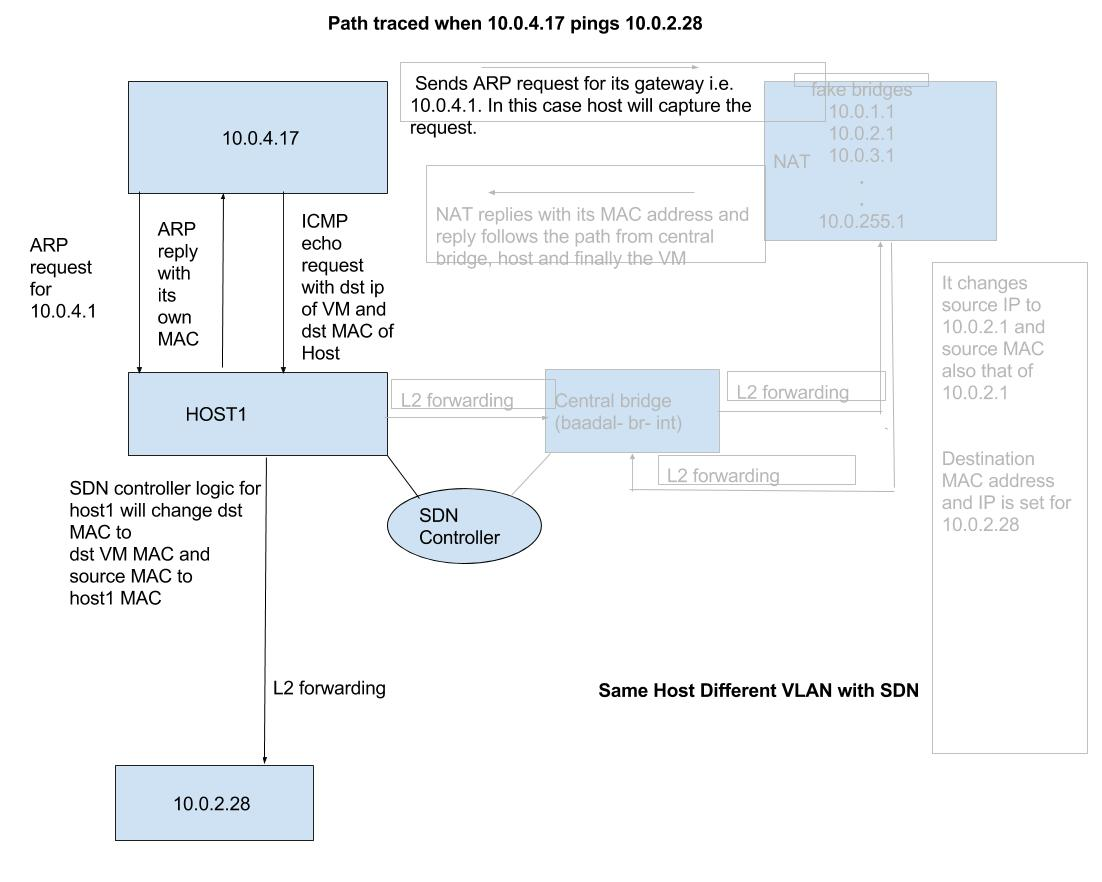
\includegraphics[width=0.9\textwidth]{Samehost_differentvLan_SDN}
\end{figure}

\pagebreak

\begin{itemize}
    \item \textbf{Different host and Different VLAN} In this case host itself will reply to the ARP request, sent by the VM for its gateway. In traditional routing, this reply was generated by the NAT. But now Central bridge will come into the picture to forward the packet to the other host2 unlike previous case. The modification in the Ethernet frame here is done by the host1 only. Host2 will simply forward the packet to the destination VM.
\end{itemize}

\begin{figure}[h]
\caption{Routing in Different Host and Different VLAN using SDN}
\centering
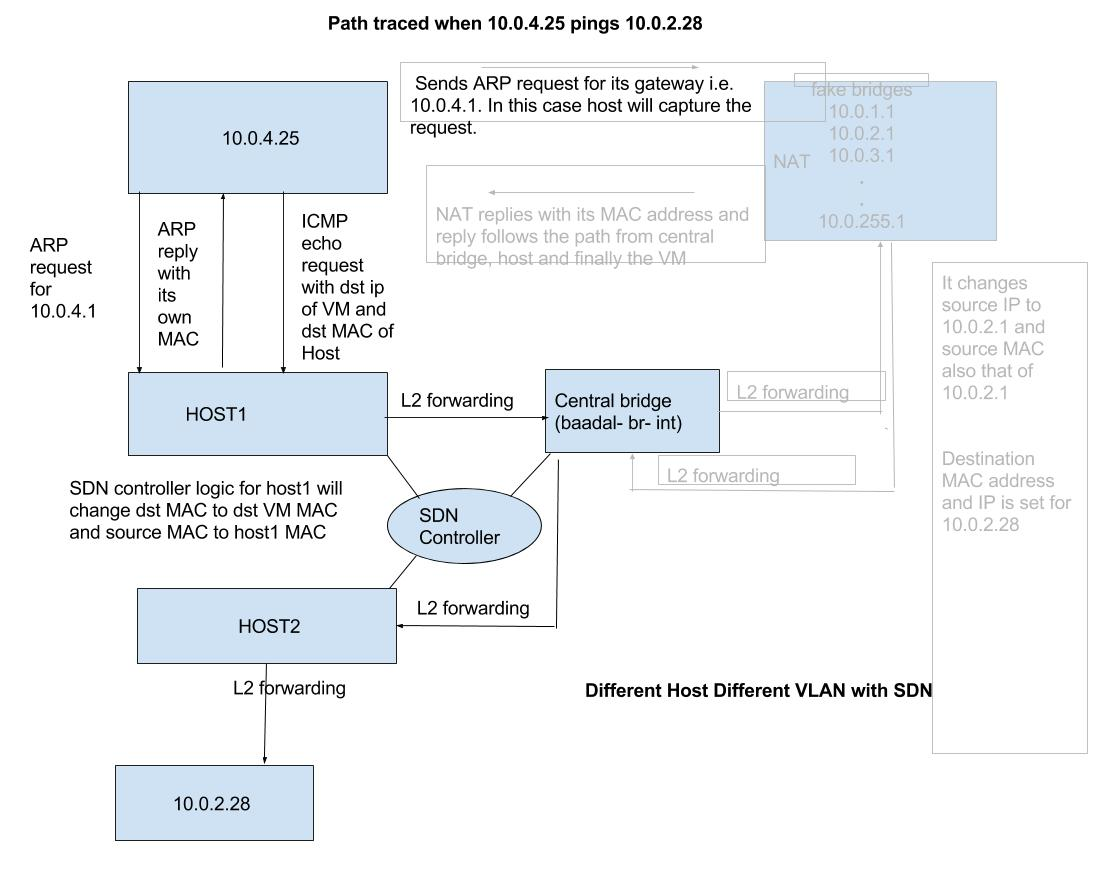
\includegraphics[width=0.9\textwidth]{Differenthost_differentvLan_SDN}
\end{figure}


\pagebreak

\begin{itemize}
    \item \textbf{Different host and Same VLAN} In this, the packet will be forwarded by the host on the basis of the MAC address to the central bridge.The central bridge will further forward it to the other host which subsequently make the packet reach destination VM.
\end{itemize}

\begin{figure}[h]
\caption{Routing in Different Host and Same VLAN using SDN}
\centering
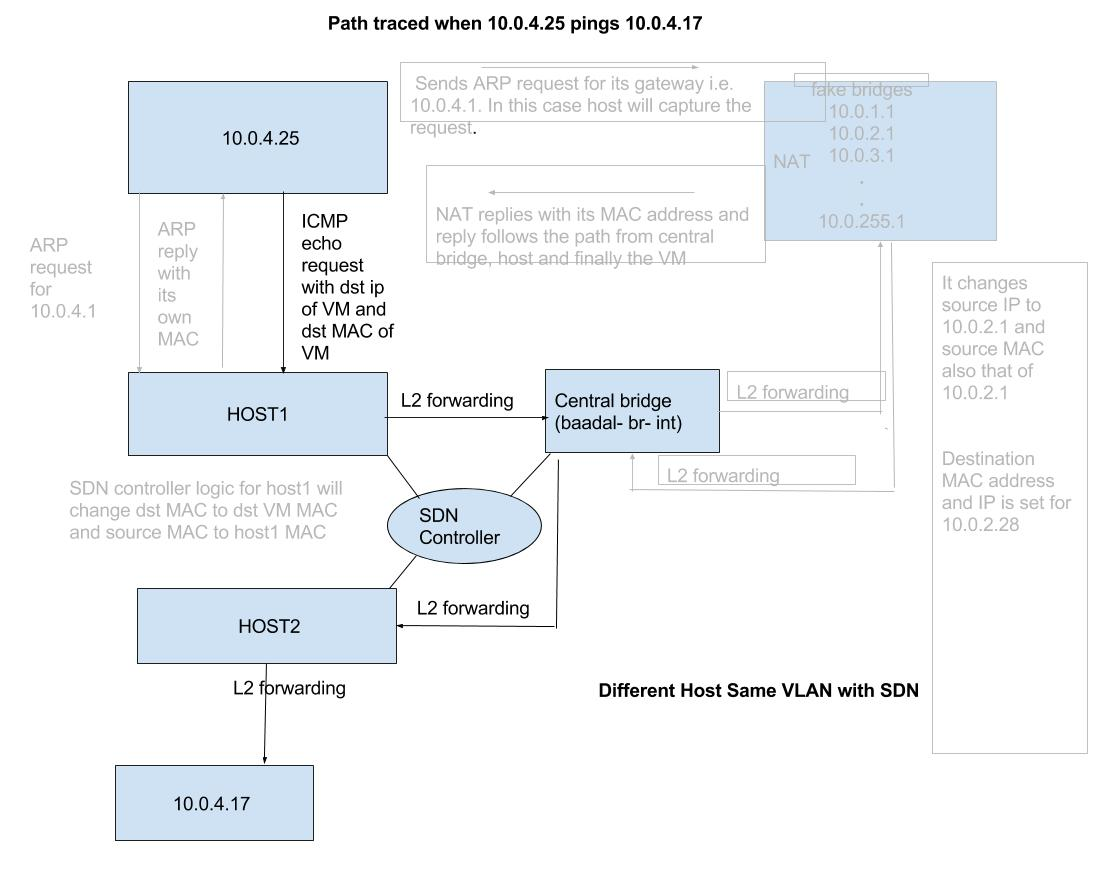
\includegraphics[width=0.9\textwidth]{Differenthost_SamevLan_SDN}
\end{figure}


% \section{Introduction to VMs consolidation application}

% \section{Major issues faced in the project}
\newpage
\section{Application pseudo code}
\begin{algorithm}[H]
\SetAlgoLined


 \If{packet type == IPv6\_TYPE}{
  Drop the packet\;
  Install flow to drop matching packets\;
  }
  \If{packet type== ARP\_TYPE}{
  \If{ARP type == REQUEST}{
    \eIf{destinationProtocolAddress is one of the gateways}{
    send reply with host's mac address\;
    don't send the packet for further processing\;
    }{
    send the packet for further processing\;
    }
  }{
  \If{ARP type == REPLY}{
    store the incoming ip to mac mapping\;
    send the packet for further processing\;
  }
  }
  }
  
  \caption{Handling arp requests at hosts}
  \end{algorithm}
  \newpage
  \begin{algorithm}
  \SetAlgoLined
  
  
  
  \If{input port = local port}{
  \If{mac corresponding to destination ip is not known}
  {
    send ARP request for destination ip\;
    wait for 100ms\;
  }
  \eIf{mac corresponding to destination ip is still not known}
    {drop the packet\;
  }{
   replace the destination mac address of the packet with the mac corresponding to the destination ip read from the table\;
  }
  \eIf{output port is known}
  {
    send the packet out\;
    install flow for all the above actions\;
  }
  {
    drop the packet\;
  }
  }
 \caption{Routing packets coming from local port of hosts}
\end{algorithm}

\newpage
\begin{algorithm}
\SetAlgoLined

\If{input port = trunk port}{
\If{output port corresponding to destination mac is not known}
  {
    send ARP request for destination ip and wait for 100ms\;
  }
  \eIf{output port is still not known}
    {drop the packet\;
  }{
   \eIf{output port is local or trunk}{
     send packet out and install flow\;
   }{
    \eIf{packet is untagged}
    {
        send packet out and install flow\;
    }{
        get policy decision between source and target ip address\;
        \If{decision == ALLOW}{
            pop vlan, send packet out and install flow\;
        }
        \If{decision == DISALLOW}{
            drop packet and install flow\;
        }
        \If{decision == DEFAULT}{
            \eIf{inter vlan routing is enabled}{
                pop vlan, send packet out and install flow\;
            }{
                \If{vlan tag of packet is same destination ip's tag}{
                    pop vlan, send packet out and install flow\;
                }{
                    drop the packet and install flow;
                }
                
            }
        }
    }
   }
  }
}
\caption{Routing packets coming from trunk port of hosts}
\end{algorithm}

\newpage
\begin{algorithm}
%\SetAlgoLined

\If{input port = access port}{
figure out if the packet is intended for the host or for any other machine\;
\eIf{destination ip is NOT of host AND destination mac is of host}{
    \If{mac corresponding to destination ip is not known}
  {
    send ARP request for destination ip\;
    wait for 100ms\;
  }
  \eIf{mac corresponding to destination ip is still not known}
    {drop the packet\;
  }{
    set the destination mac address to the mac corresponding to destination ip from the table\;
    set the source mac to host's mac\;
  }
  \If{output port is not known}{
    send ARP request for destination ip address\;
    wait for 100 ms\;
  }
}{
    \If{output port is not known}{
    send ARP request for destination ip address\;
    wait for 100 ms\;
    }
    \eIf{output port is known}{
        \If{output port is TRUNK}{
            push vlan tag, send packet out and install flow\;
        }
        \If{output port is LOCAL}{
            send packet out and install flow\;
        }
        \If{output port is ACCESS}{
            route according to inter vm policy\;
            check next page for details\;
        }
    }{
        drop packet and install flow\;
    }
}
}
\caption{Routing packets coming from access ports of hosts}
\end{algorithm}

\newpage
\begin{algorithm}
\SetAlgoLined
\If{output port is ACCESS}{
    get policy decision between source and target ip addresses\;
    \If{decision == ALLOW}{
        send packet out and install flow\;
    }
    \If{decision == DISALLOW}{
        drop packet and install flow\;
    }
    \If{decision == DEFAULT}{
        \eIf{inter vlan routing is enabled}{
            send packet out and install flow\;
        }{
            \eIf{vlan tags of source and target ip are same}{
                send packet out and install flow\;
            }{
                drop packet and install flow\;
            }
        }
        
    }
}
\caption{Routing according to inter vm policy when both input and output ports are access ports}
\end{algorithm}



\chapter{Results, Conclusion and Future Work}

%Replace \lipsum with text.
% You may have as many sections as you please. This is just for reference.

\section{Comparison of SDN based solution in terms of Bandwidth}


\section{Results for VMs consolidation application}


\section{Conclusion}

\section{Future Work}


\bibliographystyle{plain}
\bibliography{biblio}

%\appendix
%\chapter{CHAPTER NAME}

\section{SECTION NAME}
\lipsum[1]

\section{SECTION NAME}
\lipsum[2]

\end{document}
	